\documentclass[conference]{IEEEtran}
\IEEEoverridecommandlockouts
% The preceding line is only needed to identify funding in the first footnote. If that is unneeded, please comment it out.
\usepackage{cite}
\usepackage{amsmath,amssymb,amsfonts}
\usepackage{algorithmic}
\usepackage{graphicx}
\usepackage{textcomp}
\usepackage{xcolor}
\usepackage{adjustbox}
\usepackage{tabularx}
\usepackage{tabu}
\usepackage{fourier} 
\usepackage{array}
\usepackage{makecell}
\usepackage{verbatim}
\usepackage{kotex}
\graphicspath{ {./images/} }

\def\BibTeX{{\rm B\kern-.05em{\sc i\kern-.025em b}\kern-.08em
    T\kern-.1667em\lower.7ex\hbox{E}\kern-.125emX}}
\begin{document}

\title{Brain Engraver - Vocabulary Learning Program Based on Forgetting Curve\\
{\footnotesize \textsuperscript{*}Group Name: The Teachers}

}

\author{\IEEEauthorblockN{1\textsuperscript{st} Young Jae OH}
\IEEEauthorblockA{\textit{Information Systems} \\
\textit{Hanyang University}\\
Seoul, South Korea \\
jashealer@naver.com}
\and
\IEEEauthorblockN{2\textsuperscript{nd} Dong Hee Lee}
\IEEEauthorblockA{\textit{Information Systems} \\
\textit{Hanyang University} \\
Seoul, South Korea \\
ryu0315360@gmail.com}
\and
\IEEEauthorblockN{3\textsuperscript{rd} Antoine Maffeis}
\IEEEauthorblockA{\textit{Electronic Engineering} \\
\textit{Hanyang University/ESILV}\\
Seoul, South Korea \\
maffeisantoine@gmail.com}
\and
\IEEEauthorblockN{4\textsuperscript{th} Sébastien Yung}
\IEEEauthorblockA{\textit{ Electronic Engineering} \\
\textit{Hanyang University/ESILV}\\
Seoul, South Korea \\
sebastienclarkyung@gmail.com}
}

\maketitle

\begin{abstract}
It goes without saying that traditional text-based memorizing technique is not effective. The problem behind memorizing words is that memorized words are often stored in the short-term memory of our brain, not in the long-term memory section. In practice, combining learning activity with a forgetting curve has been proved to substantially improve the effectiveness of studying. In this paper, we make the first study to enhance human memorization via the forgetting curve using the NUGU AI speaker. The user goes through two stages, which are the learning and test stage. In the learning stage, the user repetitively learns the vocabulary of choice and the NUGU AI speaker helps this process by reading the word \begin{comment}and showing the nuance of the word with color\end{comment}. In the test stage, users are being tested with word lists, which comprises newly learned vocabularies and the words that have been selected by the forgetting curve technique.
\end{abstract}

\begin{IEEEkeywords}
NUGU AI speaker, forgetting curve, memorization
\end{IEEEkeywords}

\section{Introduction}
The most basic and crucial part of learning a foreign language would be “memorizing words”. To illustrate, we are frequently required to memorize a huge amount of vocabulary for a specific certificate or test. The traditional memorizing method, which is based on text, is neither efficient nor effective. To give you a clearer image, even if we memorize the words, it is very likely to be “stored” via the short-term memory, rather than the long-term memory. The shortcomings of this method are particularly evident when one needs to learn the pronunciation of words that are heard and spoken. In order to solve this issue, this paper aims to overcome the limitations of traditional word memorization methods with Brain Engraver which is run under the NUGU AI Speaker. Users using our software go through two stages every day, and these two stages are the learning stage and the test stage. In the learning stage, the user tries to learn and memorize the set of preselected words. The word set to learn can be selected from multiple word sets pre-stored in the application, users can add words directly to the word set, or even create a whole new set. When the learning stage begins, the NUGU AI speaker repeatedly reads the pronunciation and meaning of the word and then moves on to the next word after the user’s preset time. The number of words that are carried out in a single study(stage) is also set by the user himself. \begin{comment}When a speaker reads the meaning and pronunciation of the word, a light on the speaker flicks up, showing the subtle nuance of the vocabulary via colored light.\end{comment} 
In the second, testing stage, the user answers the meaning of the word spoken by the NUGU AI speaker. The test word set consists of a new set of words memorized by the user and a list of previously memorized words. It calculates the review cycle by the forgetting curve and gives a question that the user will be most likely to be forgotten. This prevents unnecessary repetition of quizzes and helps you to move your short-term-memorized vocabulary into long-term memory. Furthermore, the word is specified into sensory memory, short-term memory, and long-term memory categories, thereby creating a new review word list the following day.

\begin{table}[htbp]
\caption{Role Assignments}
\begin{center}
\begin{tabular}{ | c | c | c | } 
\hline
\textbf{\textit{Role}}& \textbf{\textit{Name}}& \textbf{\textit{Task}} \\
\hline
User& \makecell{Antoine\\Maffeis}& \makecell{Predicts the user’s needs in the\\ user’s point of view. Also searches\\existing related studies and\\compares it with the project.}   \\
\hline\
Customer& \makecell{Sébastien\\Yung}& \makecell{Checks if the application is\\ tempting enough for customers.\\
Also checks if the requirements\\are sufficient or not.}\\
\hline
\makecell{Software\\Developer}& \makecell{Dong Hee\\LEE}& \makecell{Determines what languages to use\\for the\ project and works on the\\actual software development.\\ Mostly puts focus on actualizing\\the requirements.}   \\
\hline
\makecell{Development\\Manager}& \makecell{Young Jae\\OH}& \makecell{Manages the whole project\\Sums the user’s and customer’s needs\\and reflects it into the program. Evaluates\\the software features and\\helps software developer coding.}\\
\hline
% \multicolumn{1}{1}{$^{\mathrm{a}}$Sample of a Table footnote.}
\end{tabular}
\label{tab1}
\end{center}
\end{table}

\section{Requirements}

\subsection{Mobile application}

\begin{enumerate}
% \item The purpose of this application is to visually show the users to select the word set, customize their own word set, and to see their progress on memorizing the selected words. On top of this, this mobile application is connected to the external server in order to fetch and pass data to the speaker.
\item The purpose of this application is to visually show the users wordset and subwordset. 

\item It will run on Android OS.
\item Login screen
    \begin{enumerate}
    \item ID and password are required to access the user-specific database.
    %\item There should exist a way for the users to request a new password in case they forgot their own password.
    \item It should offer a ‘stay logged in’ checkbox for user convenience.
    \item It should be able to make a brand-new account for the newcomers.
    \item In the login process, the application should show the users a loading page.
    \end{enumerate}
\item Word set
    \begin{enumerate}
    \item The users should be able to see specific types of word sets to learn. These word sets consist of Sub-word set(Chapters).
    % \item If the user requires to make a whole new word set or edit existing word sets, they should be able to add, delete the specific word set of their choice.
    % \item There should be a checkbox next to these word sets in order to show that the user has already learned or currently learning the specific word set.
    \end{enumerate}
\item Sub-word set
    \begin{enumerate}
    \item Inside the word set, there should exist a list of sub-words sets to learn (e.g., Chapter 1, Chapter 2…)
    % \item The user should be able to add, delete the specific sub-word set of their choice.
    % \item There should be a checkbox next to these sub word sets in order to show that the user has already learned or currently learning the specific sub word set.
    % \item The checkbox changes into green if the user finished the whole process; learning stage and the test stage, and into yellow if the user only finished the learning stage.
    \end{enumerate}
\item Word
    \begin{enumerate}
    \item Inside the sub-word sets, the users should be able to see the list of words.
    \item This word list comprises ‘spelling’, ‘meaning’. 
    % ‘play button’ which plays the pronunciation of the word. 
    % \item The user should be able to add, delete the specific word of their choice.
    \end{enumerate}
\item Forgetting Curve
    \begin{enumerate}
    \item The application specifies the words into a new group regarding the current position of words in the forgetting curve.
    \item List of to-be-tested words are made regarding the aforementioned information. 
    \end{enumerate}
% \item Settings
%     \begin{enumerate}
%     %\item Users should be able to choose how many words to train for a day.
%     \item Users should be able to choose the training time. More specifically, it should be possible to choose how much for the speaker to repeat the words.
%     \item Users should be able to manage the lights. They can choose whether to turn on or turn off the light. 
%     \end{enumerate}
\end{enumerate}



\subsection{Speaker}    
\begin{enumerate}
\item Learning Stage
    \begin{enumerate}
    % \item The speaker should repeat the words and show the color nuance with the led light.
    % \item In the learning stage, the traditional red(negative) to green(positive) light spectrum will flick up showing the subtle nuance of the word itself.
    \item The speaker should repeat the words three times in 1.6 seconds interval.
    \item The speaker should be able to send the progression rate to the mobile application.
    \end{enumerate}
\item Test stage
    \begin{enumerate}
    \item The speaker should read only the word, and get meaning as an input from the user.
    % \item If the answer corresponds with the original meaning of the word, green light flicks, and red light flicks otherwise.
    \item If the user wishes to know the correct meaning of the answer, the user can always check the mobile application.
    \item The speaker should send the result; correctly-answered word list and incorrectly-answered word list to the mobile application for the data process after.
    \item The speaker should be able to send the progression rate to the mobile application.
    \end{enumerate}
\end{enumerate}

\subsection{Server}    

\begin{enumerate}
\item Application
    \begin{enumerate}
    \item When the user chooses a word set, the ‘current-learning list’ gets updated.
        \begin{enumerate}
        \item Vocabularies from Chapter 1 goes into the ‘current-learning list’ by default.
        \item The number of words going into the ‘current-learning list’ depends on the number the user set in the setting page of the mobile application.
        \end{enumerate}
    \item Add user’s own word set
        \begin{enumerate}
        \item If the user adds or deletes a word in the word set, update it into the DB.
        \item When the user adds a word in the word set, the application updates it into the DB.
        \item If the user deletes its own custom word set, delete it from the DB.
        \end{enumerate}
    \item Editing pre-existing word set
        \begin{enumerate}
        \item If the user adds or deletes a word in the pre-existing word set, update it into the DB.
        \item When the user adds a word in the pre-existing word set, the application updates it into the DB.
        \item If the user deletes the pre-existing word set, delete it from the DB.
        \end{enumerate}
    \end{enumerate}
\item Speaker
    \begin{enumerate}
    \item Learning Stage
        \begin{enumerate}
        \item Server sends the NUGU speaker ‘current-learning list’.
        \item When the user finishes the learning stage, update the checkbox into yellow.
        \item After the test stage, fetch the correctly-answered word list and the incorrectly-answered word list and send it to the server.
        \end{enumerate}
    \item Test Stage
        \begin{enumerate}
        \item When the user finishes the test stage, update ‘to-be-tested list’.
        \item The incorrectly-answered word list is automatically added into the ‘to-be-test list’.
        \item Copy the ‘current-learning list’ into ‘previous-word list’.
        \item Empty the ‘current-learning list’.
        \item Correctly-answered word list is first processed via the forgetting curve algorithm and then added into the ‘to-be-tested list’.
        \end{enumerate}
    \end{enumerate}
\end{enumerate}




\section{Development environment}

\subsection{Choice of software development platform}
\begin{enumerate}
    \item For our software development, we will be using mac OS Catalina, Windows 10, and Linux Ubuntu. Windows 10 will be used for developing the mobile application because it is more compatible than any other OS with the software we will be using for application development. Mac OS will be used for the server-side since it is based on Unix. For the server, we are using the AWS EC2 Ubuntu(20.04) free-tier instance.
    \item Programming Language
    \begin{enumerate}
    \item Python 3.8.3
        \begin{itemize}
            \item We are using python for the server-side and the glue language between the mobile application and the AWS server. We chose Python because it is one of the most popular programming language for developing an artificial-intelligence-related-program. Moreover, it can be run on various OS, including Microsoft Windows, Mac OS, and Linux OS. The only drawback that we came to realize was the running speed of the code. If we need a faster speed of the program, we will modularize some of the code into C or C++ code in order to achieve the required speed.
        \end{itemize}
    \item Flask
        \begin{itemize}
            \item On top of python, we will be using Flask framework for the server. We are going to construct a server with AWS EC2 Ubuntu, and control it with Python and Flask framework. Flask is famous for its lightness, simplicity, and speed. Before choosing Flask, we had to decide whether to use Flask or Django. Django also seemed to be a great choice of framework, but the fact that we were using AWS, which has many limitations, we decided on using Flask rather than Django.
        \end{itemize}
        % \item JavaScript
        %     \begin{enumerate}
        %         \item Since react-native can render codes written in JavaScript, we will be using JavaScript for the main language for building the mobile application. Moreover, it would be a good choice to choose JavaScript for both back-end and front-end of the mobile application.
        %     \end{enumerate}
        % \item Node.js
        %     \begin{enumerate}
        %         \item Node.js also uses JavaScript for its programming language, and it is widely used language for server-side programs. Since our Brain-Engraver has a frequent number of inputs and outputs going in and out from the server to the mobile application, Node.js seemed like a wise choice. Also, react-native supports for Node.js.
        %     \end{enumerate}
        
        %%%%%%%%%%%% 어플리케이션 바꿀 것
        \item C\#
            \begin{itemize}
                \item We chose to use C\# programming language for our application development. C\# has an advantage of speed over many other languages, and it is used in Xamarin, which is a framework for application development. Moreover, we have only developed an application before with C\#, so we naturally chose C\# for our app developing langauge.
            \end{itemize}
       \item Xamarin
            \begin{itemize}
                \item Before Xamarin, in order to develop a certain application for the smartphone, Objective-C, Swift was needed for iOS applications, and Java, Scala, Kotlin was required for Andriod applications. Since for us not having enough time to study many different languages for building the mobile application which has to be runnable on both Android and iOS, we chose Xamarin for developing native apps for Andriod and iOS with same language. Furthermore, Xamarin supports C#, so we decided to use the Xamarin platform. Lastly, for the mobile application, it will run on Android 10, and iOS 14.
            \end{itemize}
        %%%%%%%%%%%% 어플리케이션 바꿀 것
    \end{enumerate}
    \item Cost Estimation
        \begin{table}[htbp]
        \caption{Cost Estimation}
        \begin{center}
        \begin{tabular}{ | c | c | c | } 
        \hline
        \textbf{\textit{Software}}& \textbf{\textit{Task Description}}& \textbf{\textit{Cost}} \\
        \hline
        AWS EC2 & \makecell{Server}& \makecell{0}\\
        \hline
        Pycharm & \makecell{Code Editor}& \makecell{0}   \\
        \hline\
        Visual Studio & \makecell{Code Editor}& \makecell{0}   \\
        \hline\
        Github & \makecell{Code Repository}& \makecell{0}\\
        \hline
        Github Pages & \makecell{Blog}& \makecell{0}\\
        \hline
        \makecell{Overleaf}& \makecell{LaTeX Documentation}& \makecell{0}   \\
        \hline
        \makecell{Visual Paradigm}& \makecell{UML tool}& \makecell{0}\\
        \hline
        % \makecell{Passport}& \makecell{Authentication middleware}& \makecell{0}\\
        % \hline
        % \multicolumn{1}{1}{$^{\mathrm{a}}$Sample of a Table footnote.}
        \end{tabular}
        \label{tab1}
        \end{center}
        \end{table}
    
    \item Information about development environment
    \begin{enumerate}
        \item Computer
        \begin{enumerate}
            \item MacBook Pro
        
            \begin{itemize}
                \item Processor: Intel Core i9, 2.4GHz octa-core
                \item Ram: 32GB 2667 MHz DDR4
                \item OS: macOS Catalina(10.15.7)
            \end{itemize}
            
            \item MacBook Air
            
            \begin{itemize}
                \item Processor: Intel Core i5, 1.6GHz dual-core
                \item Ram: 4GB 1600MHz DDR4
                \item OS: macOS Catalina(10.15.7)
            \end{itemize}
            
            \item Dell XPS 15 9570
            
            \begin{itemize}
                \item Processor: Intel Core i7-8750h, 2.20GHz
                \item Ram: 16GB 2208MHz DDR4 
                \item OS: Windows 10(10.0.18363 Numero 18363)
            \end{itemize}
            
            \item HP Spectre x360 Convertible
                \begin{itemize}
                    \item Processor: Intel Core i7-8550U, 1.80GHz
                    \item Ram: 16GB 2208MHz DDR4
                    \item OS: Windows 10(10.0.18363 Numero 18363)
                \end{itemize}
        \end{enumerate}
        
        \item Commercial Cloud Platform
            \begin{itemize}
                \item Amazon Web Services(AWS) EC2, Ubuntu focal 20.04 (free-tier)
            \end{itemize}
        
    \end{enumerate}
\end{enumerate}
    
\subsection{Software in use}
\begin{enumerate}
    \item Memo Review
        \begin{figure}[h]
            \centering
            \hfill
            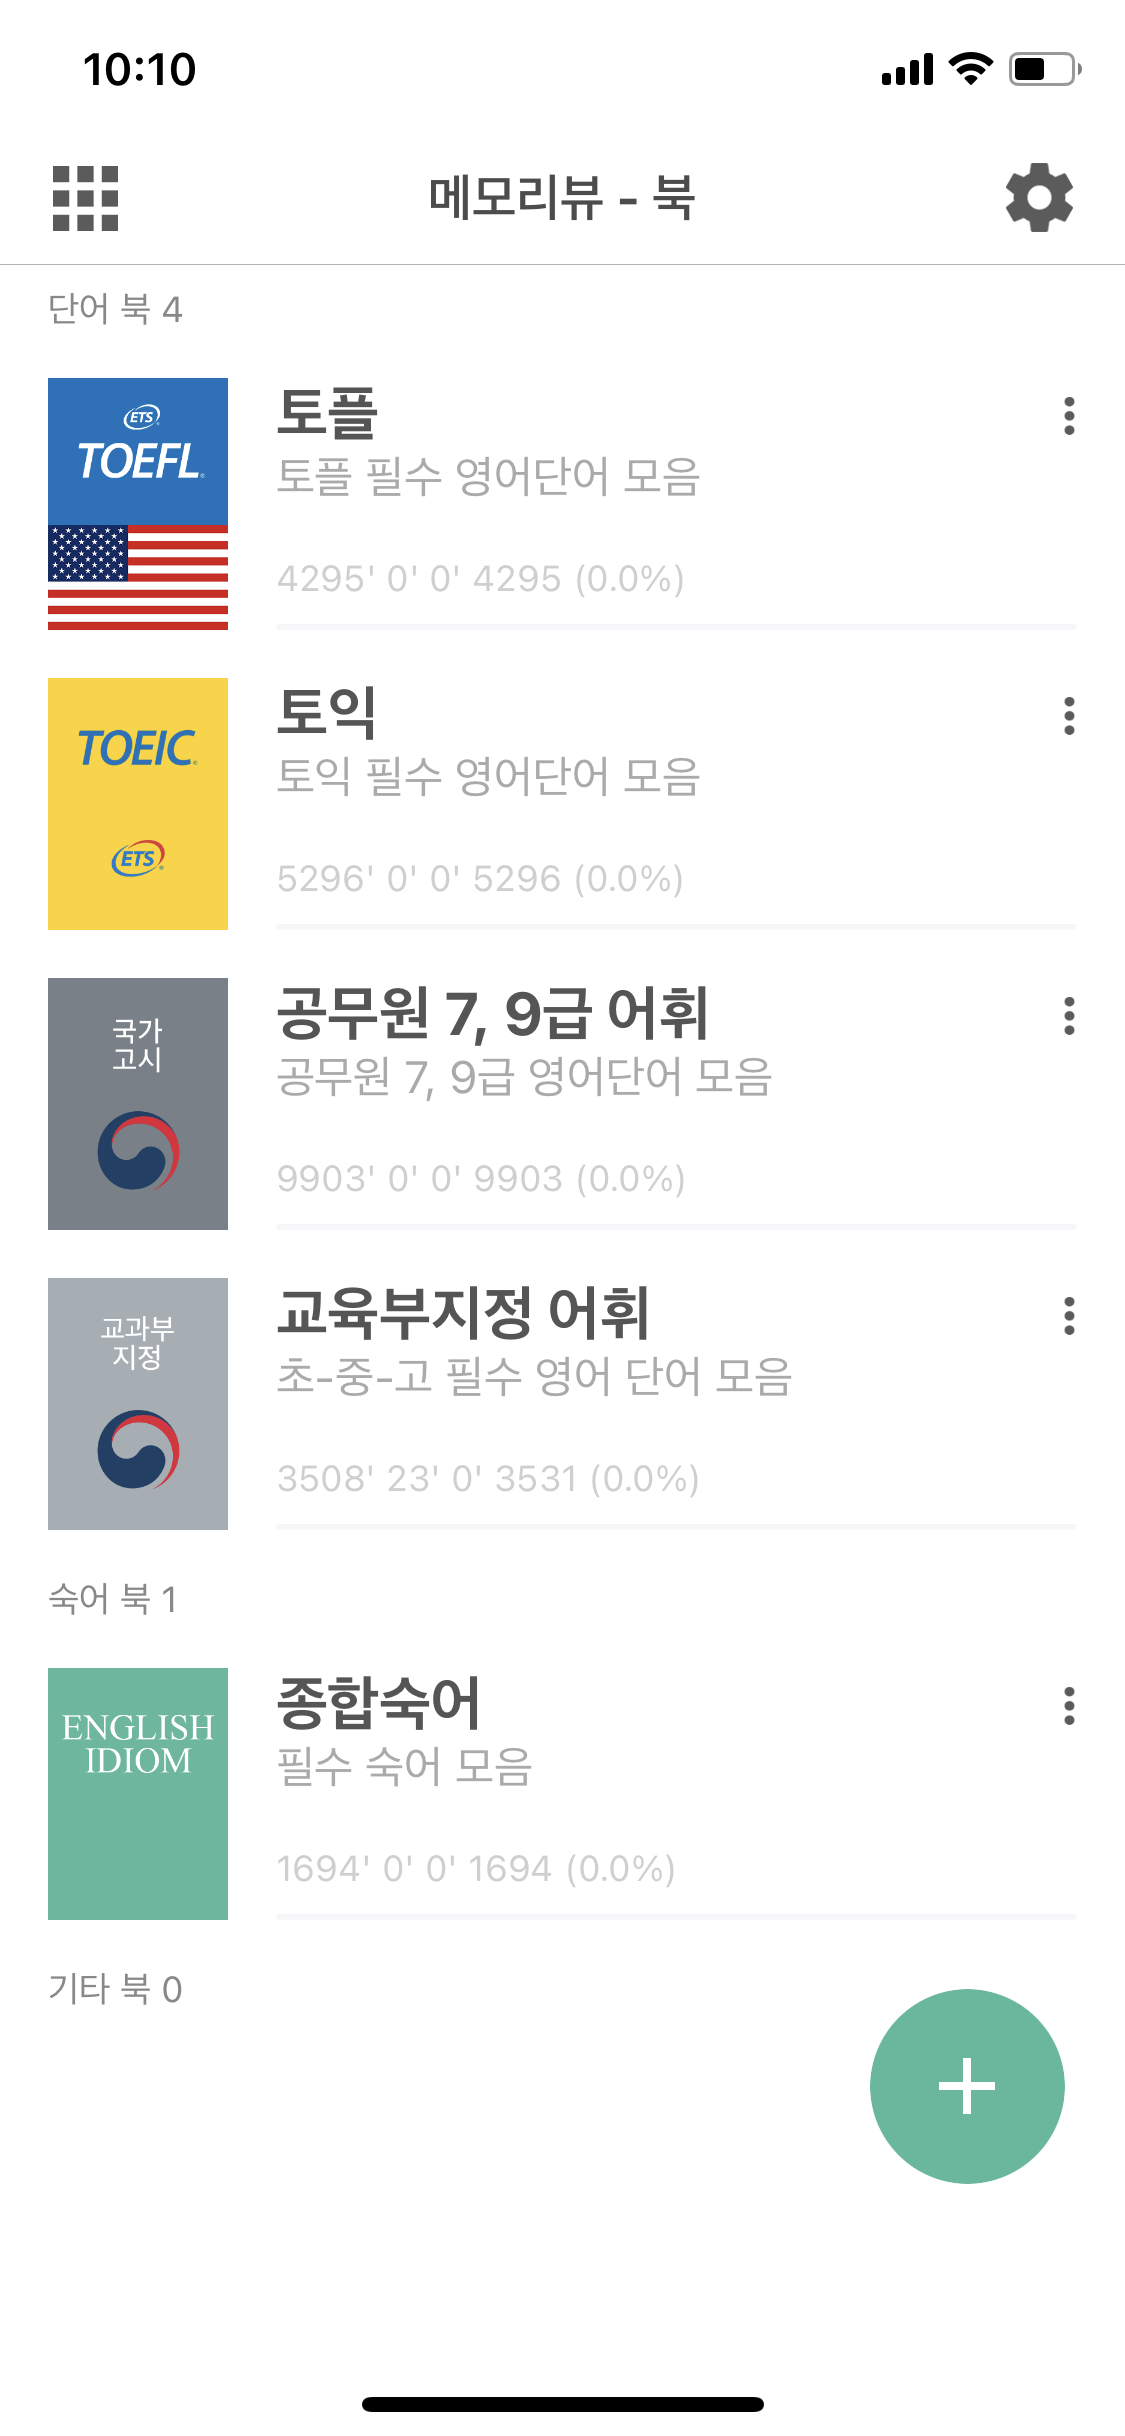
\includegraphics[width=3.5cm, height=7cm]{images/memoreview1.PNG}
            \hfill
            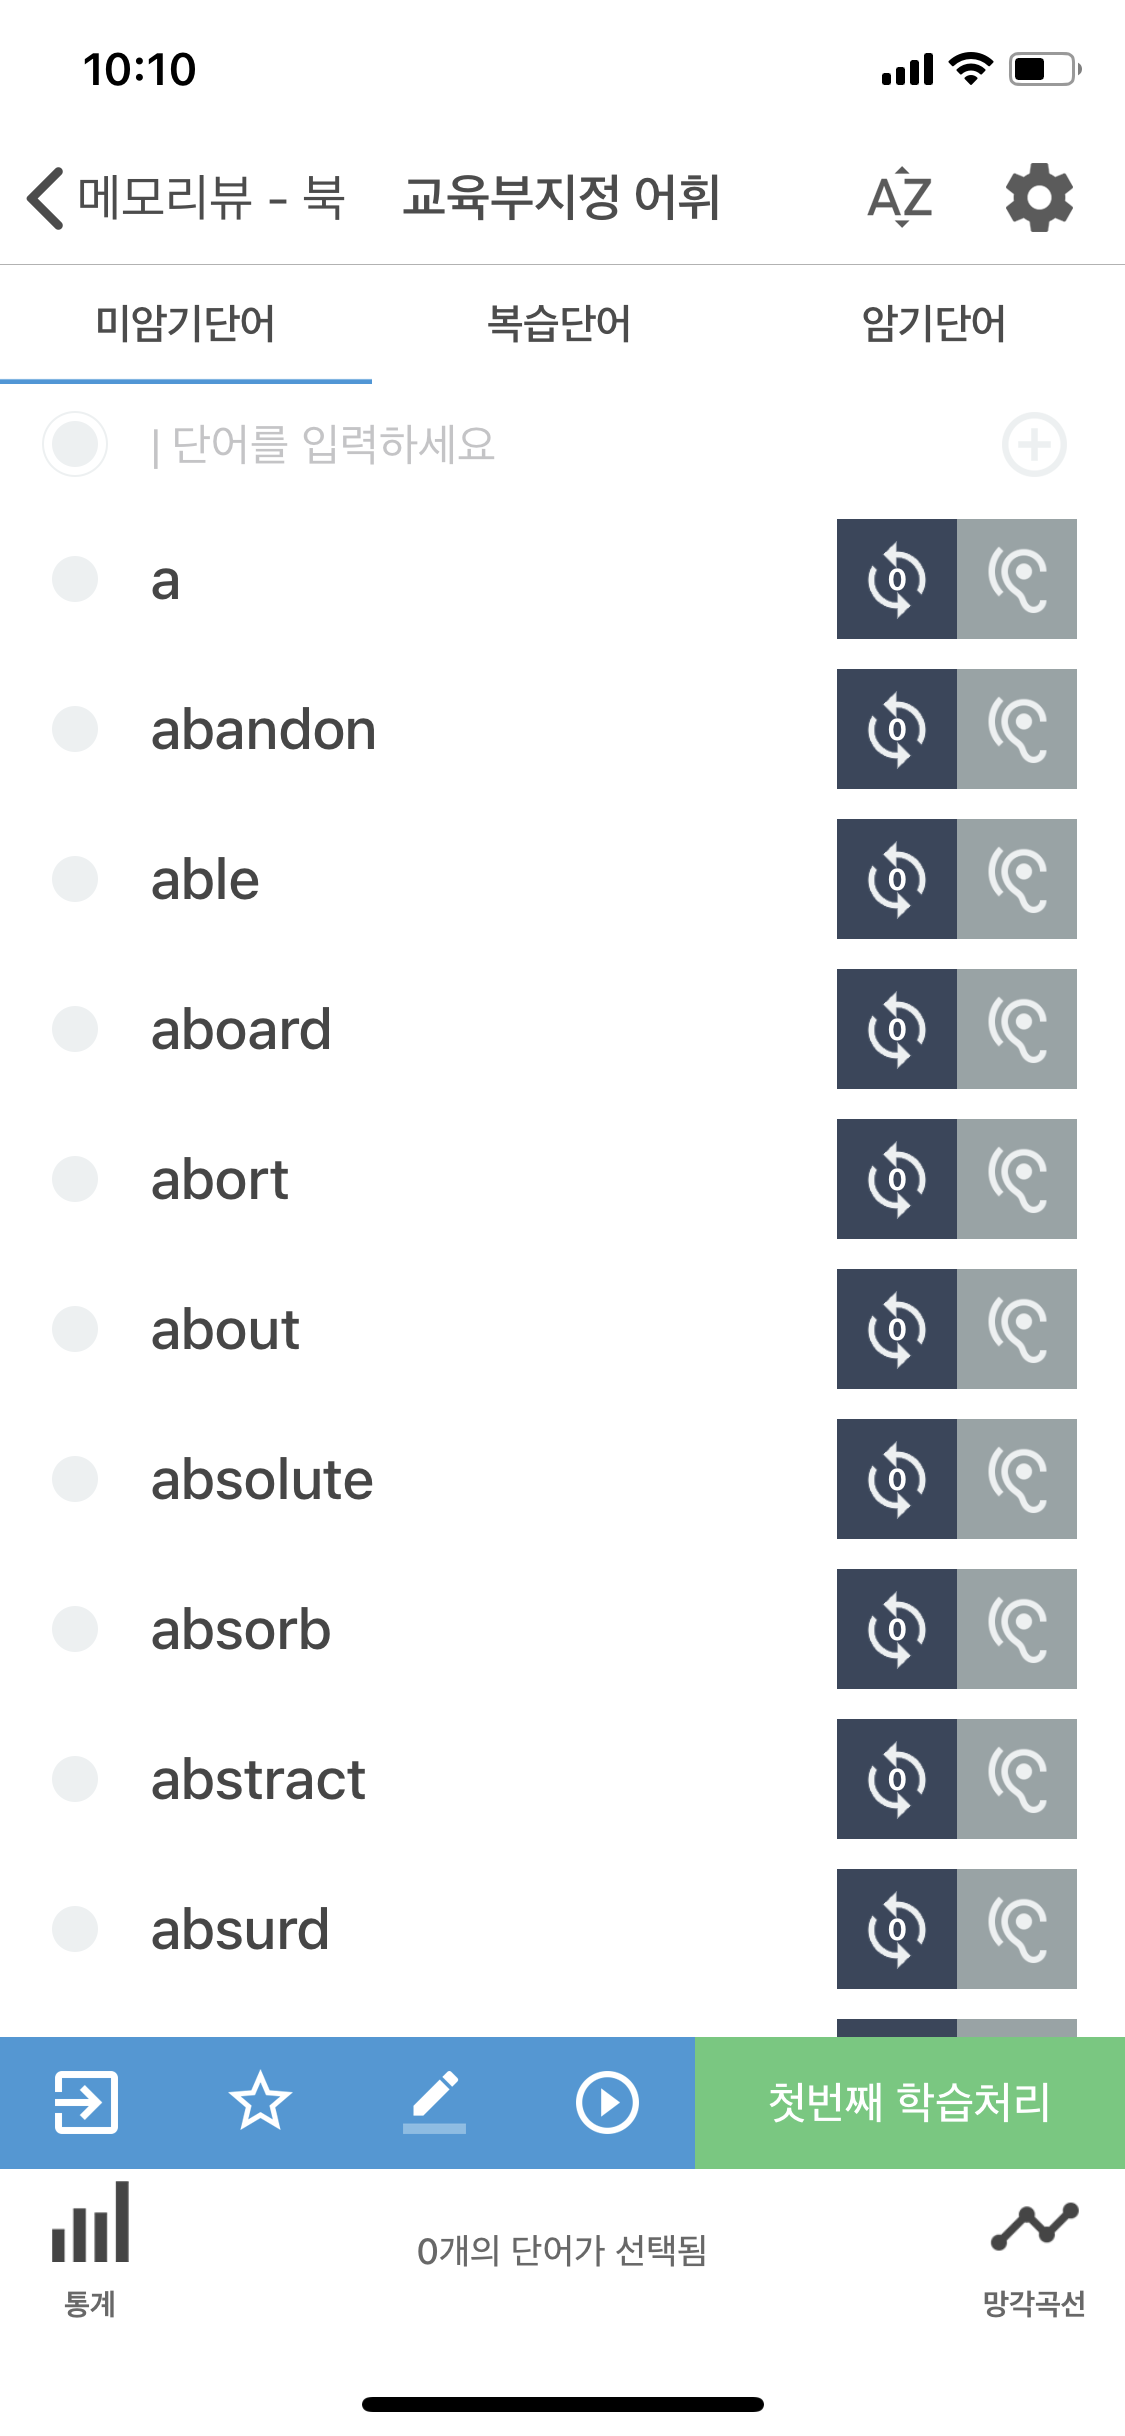
\includegraphics[width=3.5cm, height=7cm]{images/memoreview2.PNG}
            \hfill
            \caption{Memo Review}
        \end{figure}
        \begin{itemize}
            \item Rating: 2.8 (6 ratings)
            \item Feature: Helps the user to memorize vocabularies with various learning methods such as "listen-and-write" and "word card". It also shows vocabularies on human forgetting curb.
            \item Difference: This application does not support the test stage like Brain-Engraver. We compute the "likely-to-be-forgotten-words" based on test results with the human forgetting curve algorithm.
            \item Review: There are only six reviews, and most of them said it is a waste of money because of its slow loading.
        \end{itemize}
    \item Memorize.ai: Learn Lazily
        \begin{figure}[h]
            \centering
            \hfill
            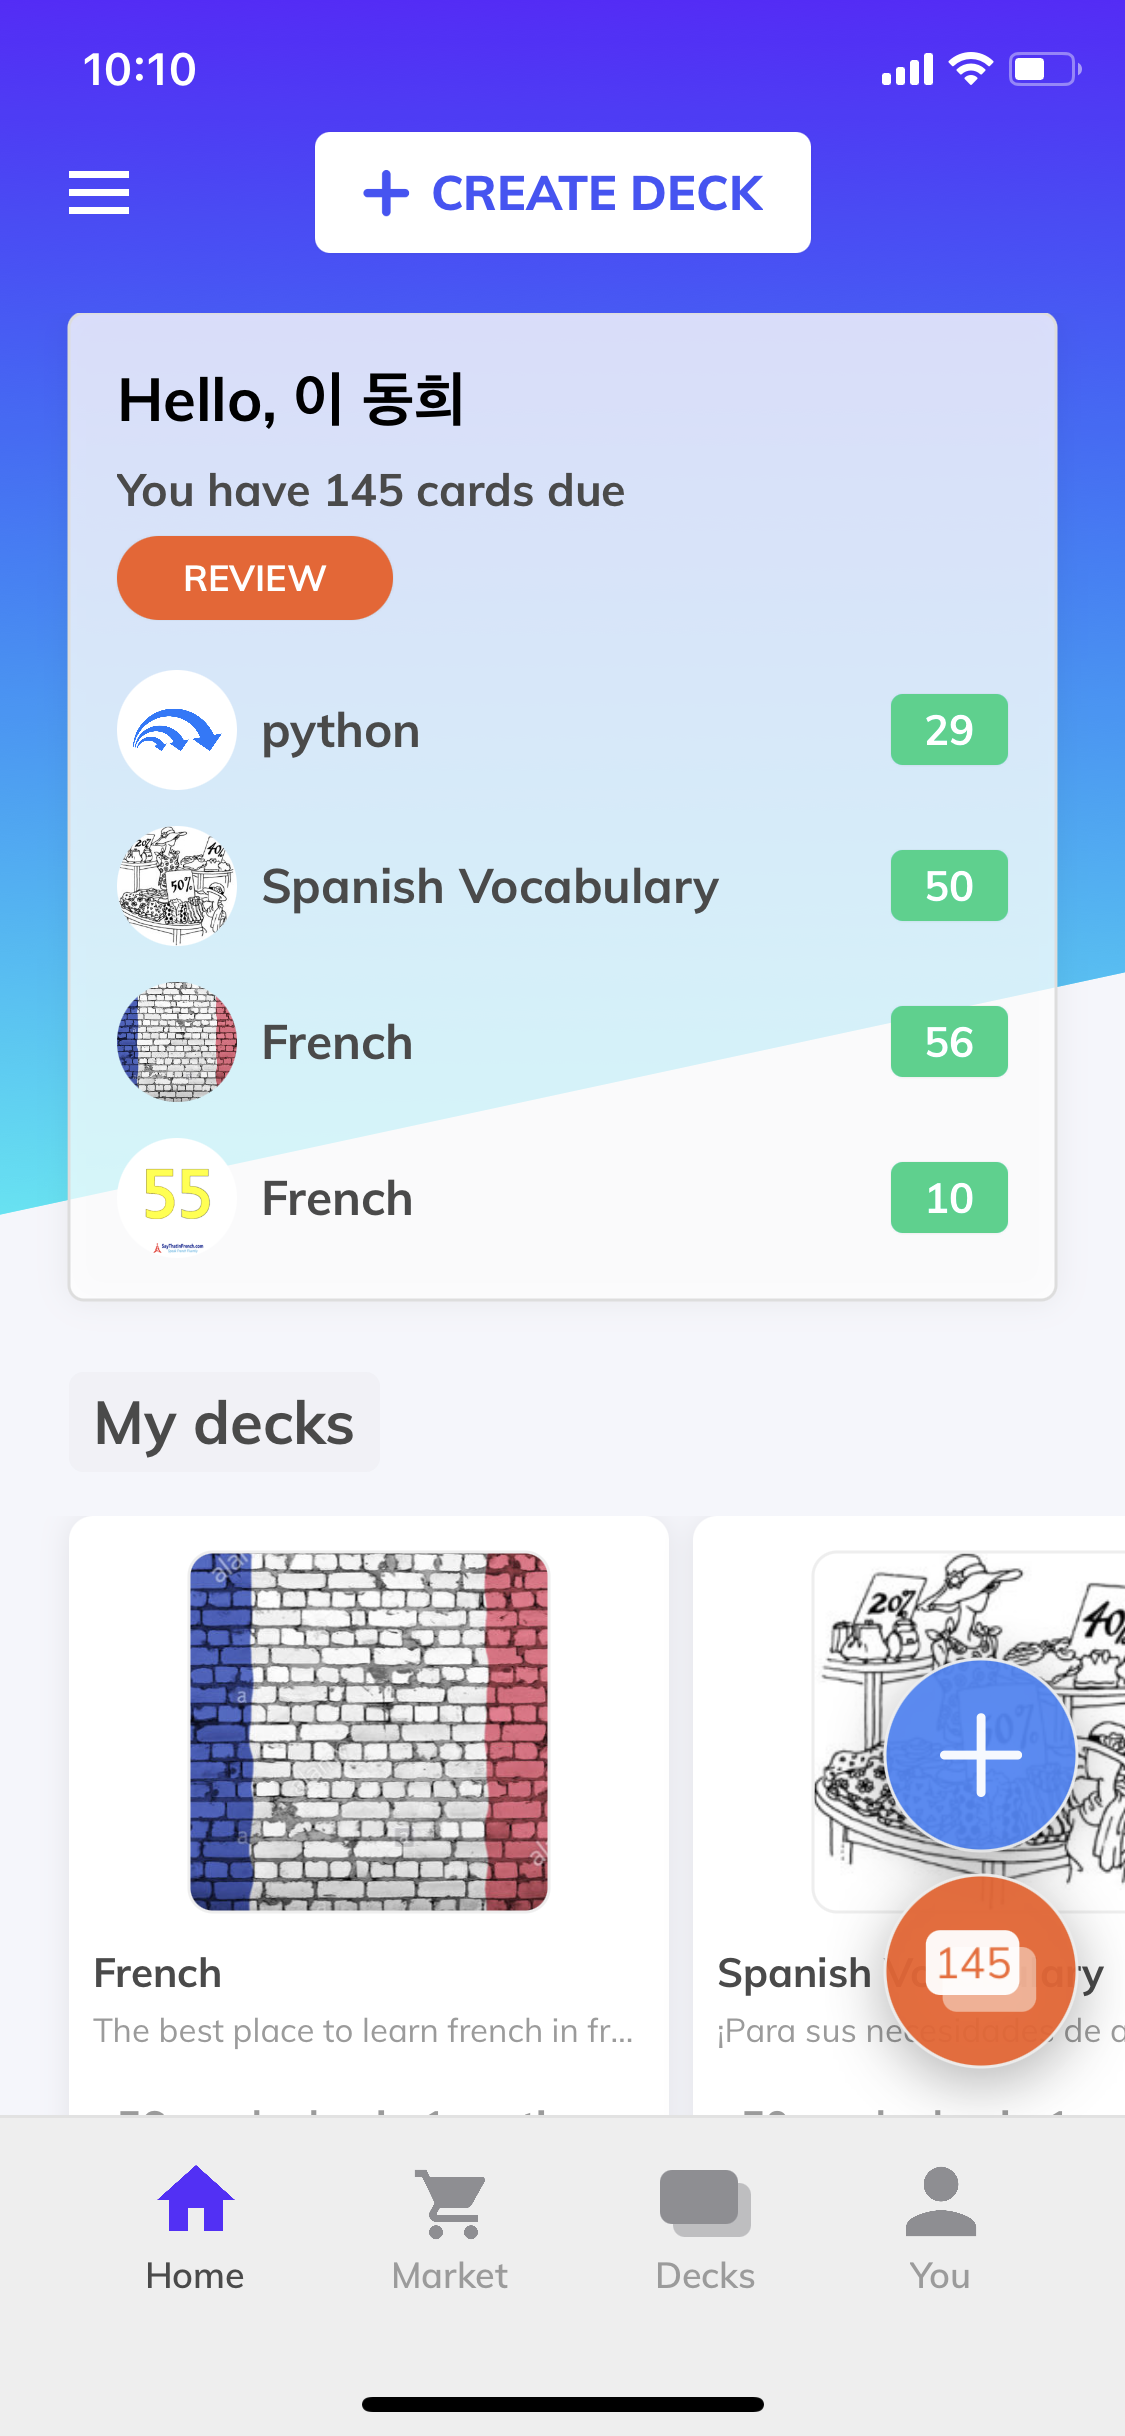
\includegraphics[width=3.5cm, height=7cm]{images/memorizeai1.PNG}
            \hfill
            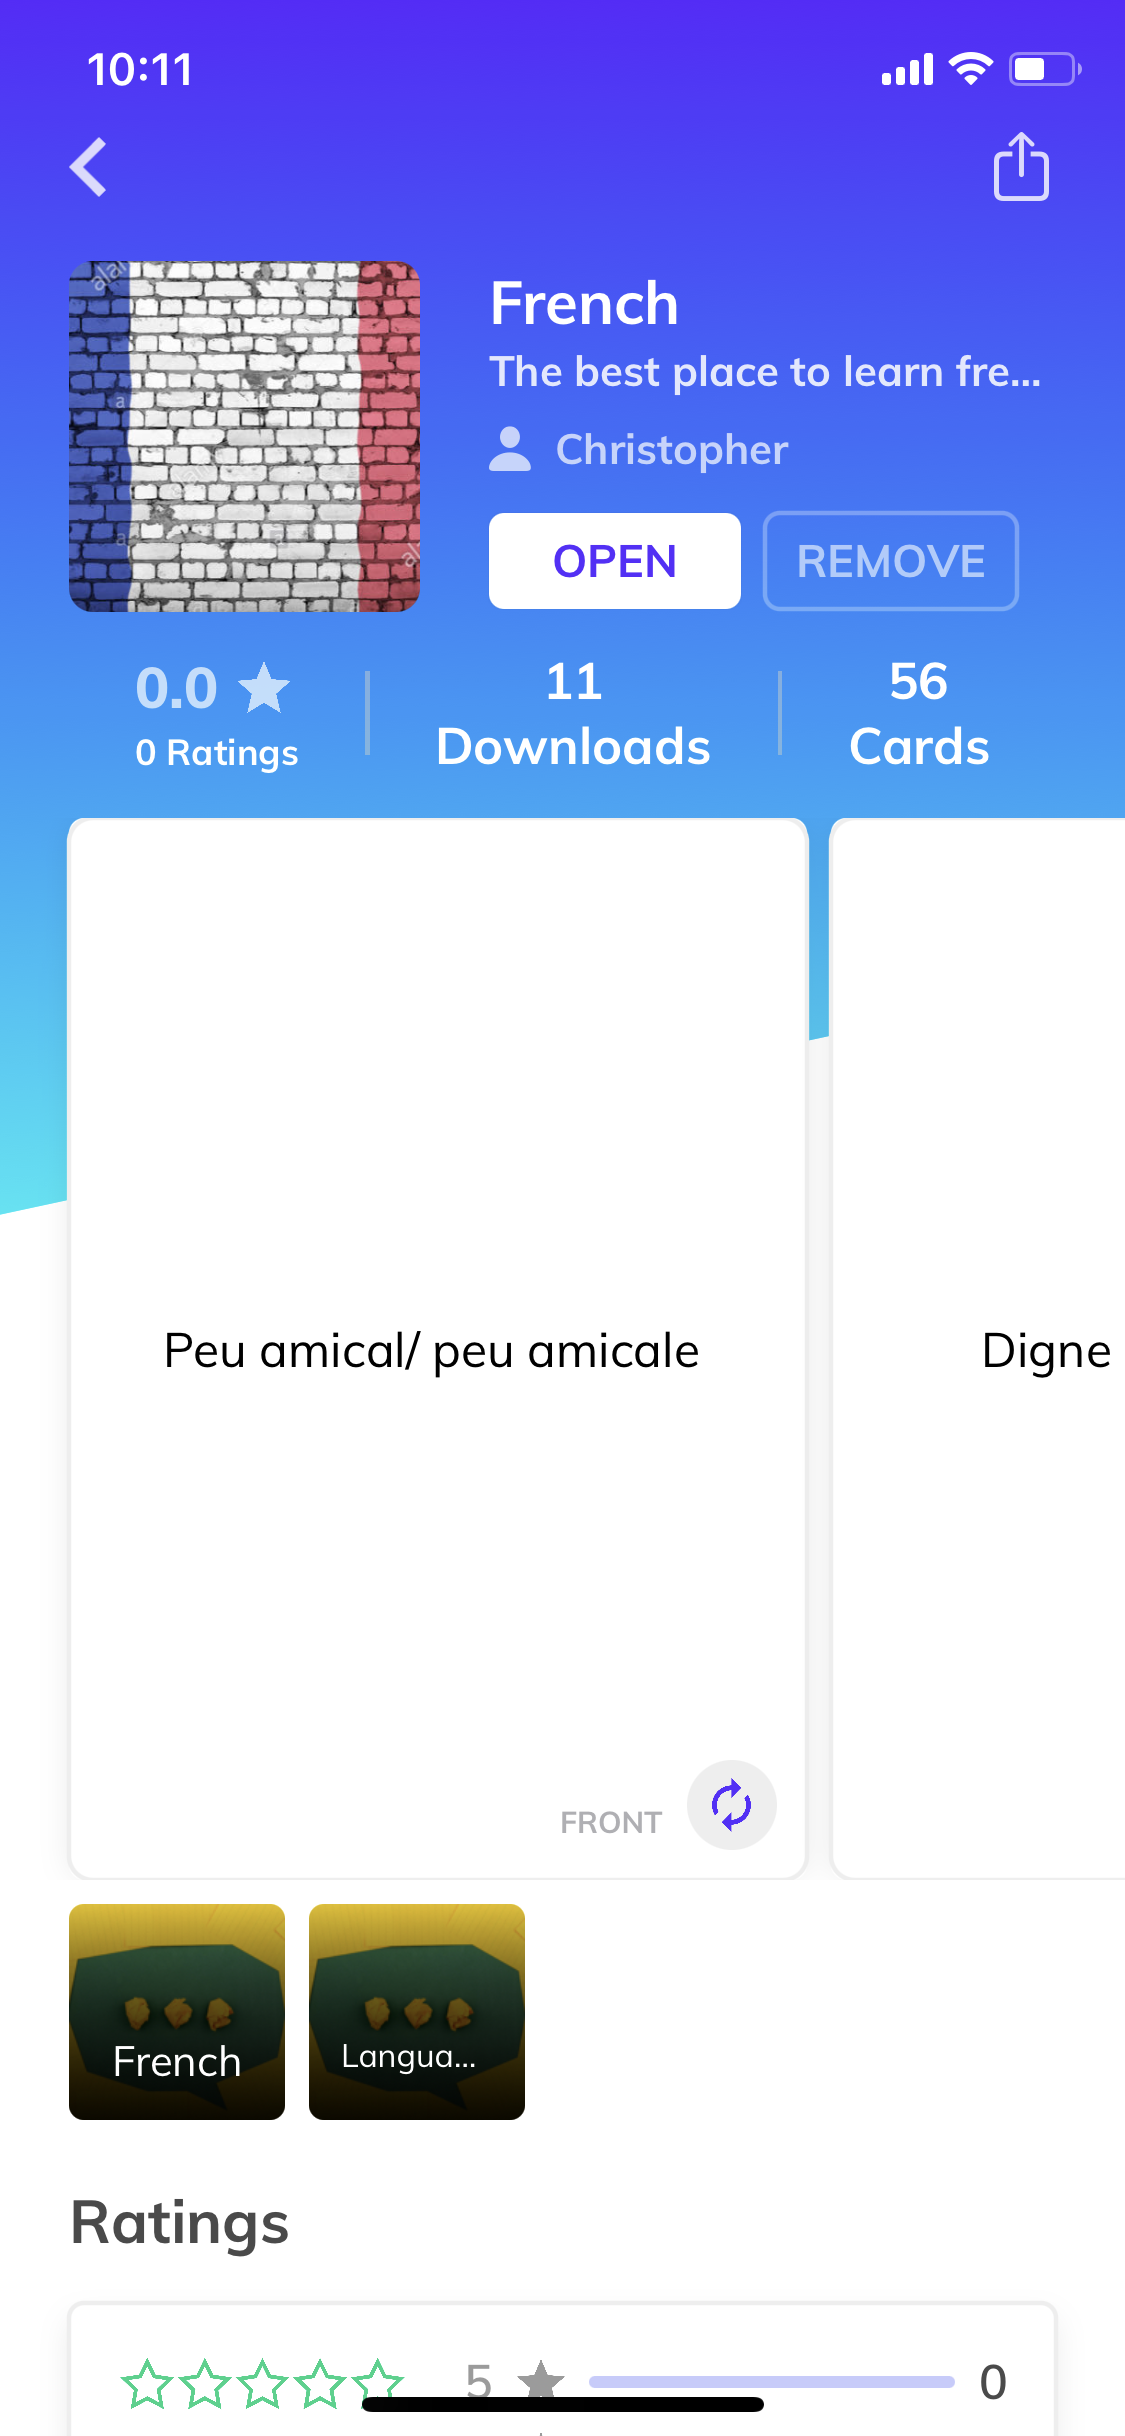
\includegraphics[width=3.5cm, height=7cm]{images/memorizeai2.PNG}
            \hfill
            \caption{Memorize ai}
        \end{figure}
        \begin{itemize}
            \item Rating: 5.0 (6 ratings)
            \item Feature: It uses artificial intelligence(they do not give specific detail about what algorithm or what technique they used for this application). It supports a feature called "Spaced Repetition". This application supports LaTeX, and code editors. 
            \item Difference: This application does not use human forgetting curve algorithm.
            \item Review: 5 out of 6 reviews said it was good, but 1 of the review claimed that it crashes consistently.
        \end{itemize}
    \item Research Paper: A Memorizing Model of Effective English Study by Kyung Lan Kim
        \begin{itemize}
            \item It goes on to detail about the fact that memorizing technique based on Ebbinghaus human forgetting curve theory is better than just hard-memorizing the words.
            \item Difference: The paper only describes the effectiveness of memorization based on the human forgetting curve. It does not provide any software-related method.
        \end{itemize}
\end{enumerate}

\subsection{Task distribution}
       \begin{table}[htbp]
        \caption{Task Distribution}
        \begin{center}
        \begin{tabular}{ | c | c | } 
        \hline
        \textbf{\textit{Name}}& \textbf{\textit{Task Description}} \\
        \hline
        Young Jae OH & \makecell{Playbuilder, backend}\\
        \hline
        Dong Hee LEE & \makecell{Playbuilder, backend}   \\
        \hline\
        Antoine  Maffeis & \makecell{App frontend, App backend}   \\
        \hline\
        Sébastien  Yung & \makecell{App frontend, App backend}\\
        \hline
        % \multicolumn{1}{1}{$^{\mathrm{a}}$Sample of a Table footnote.}
        \end{tabular}
        \label{tab1}
        \end{center}
        \end{table}






\section{specifications}

\subsection{Mobile Application}
%\begin{figure*}[h]
%    \centering
%    \hfill
%    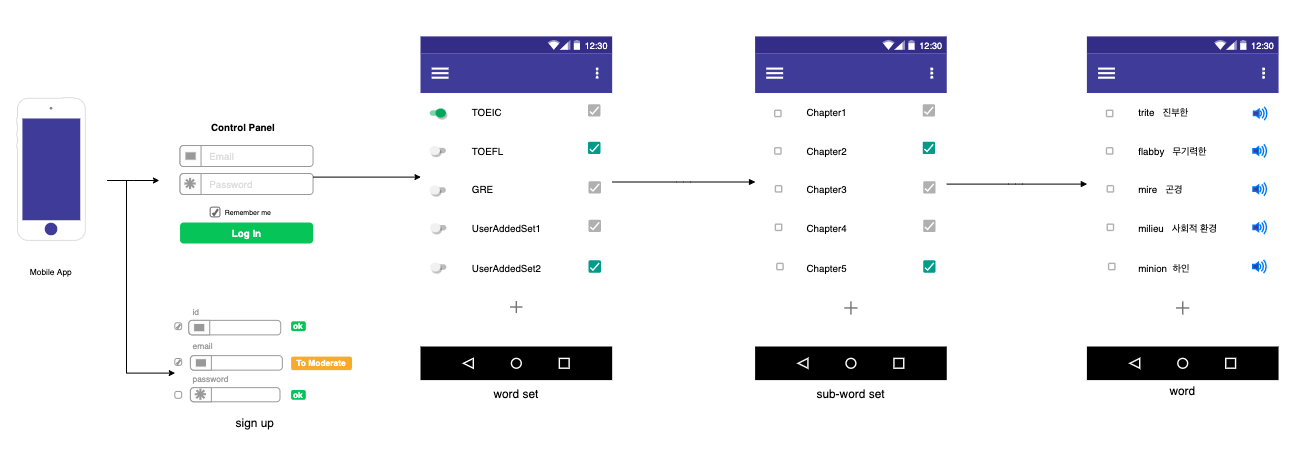
\includegraphics[width=\textwidth,height=6cm]{images/diagram_app.png}
%    \hfill
%    \caption{Mobile Application Diagram}
%\end{figure*}
\begin{enumerate}
    \item Login Screen
    \begin{enumerate}
        \item Create Account
            \begin{enumerate}
                \item Input Name, ID, PW, PW verification, E-mail
                \item Password should be 4-16 letters, mixture of English and number.
                \item If PW and PW verification field matches, create account.
                \item If PW and PW verification does not match, show message "PW does not match".
                \item after creating account, click "to Login Screen" button to login.
            \end{enumerate}
        \item Login
            \begin{enumerate}
                \item Click Login button after inputting ID and PW.
                \item If ID or PW does not exist or mismatches, reload the login screen, showing the message "ID and PW does not match"
                \item If the user checks the "keep me logged in" button, login process will no more be needed.
                \item After logging in, move to "word set" screen.
            \end{enumerate}
    \end{enumerate}
    \item Word Set Screen
        \begin{enumerate}
            \item Logout
                \begin{enumerate}
                    \item Log out to the main login screen.
                \end{enumerate}
            \item Settings
                \begin{enumerate}
                    \item Move to the settings page.
                \end{enumerate}
            \item Word Set
                \begin{enumerate} 
                    \item provide TOEIC, TOEFL, GRE word sets.
                    \item next to each word set, there is a progress checkbox. This checkbox cannot be changed by the user.
                    \item Change the checkbox into yellow if only the learning stage has been finished. Even the user only finished learning one sub-word set, the checkbox gets changed into yellow.
                    \item Change the checkbox into green if both the learning stage and test stage have been finished. Every sub-word set's test stage has to be finished in order to become color green.
                    % \item Next to every word set, there should be a delete button which deletes the word set and sends a request to the server to delete the word set.
                \end{enumerate}
            % \item Add new word set
            %     \begin{enumerate}
            %         \item The "+" button shows the user pop-up screen requiring the name of the newly-created word set.
            %         \item The name of the newly-created word set should be longer than one character.
            %         \item The "confirm" button in the pop-up screen generates a new word set and requests the server to generate a new word set to the database.
            %         \item If there already exists a word set with the same name, show message "The name is already being used".
            %         % 학습 및 테스트 할 word set 선택. 유저가 ‘진도율 체크박스’ 옆의 ‘학습 선택 체크박스’ 클릭하면 ‘학습 선택 체크박스’ 초록색으로 변함 + 팝업창 ‘학습할 단어 세트가 선택되었습니다.’ 문구.
            %     \end{enumerate}
        \end{enumerate}
        \item Sub-word set screen
            \begin{enumerate}
                \item Logout
                \begin{enumerate}
                    \item log out to the main login screen.
                \end{enumerate}
                \item Settings
                \begin{enumerate}
                    \item move to the settings page.
                \end{enumerate}
                \item Back arrow button
                \begin{enumerate}
                    \item move back to word set screen
                \end{enumerate}
                \item Sub-word set
                \begin{enumerate}
                    \item The sub word set comprises chapters of the word set.
                    \item next to each sub-word set, there is a progress checkbox. This checkbox cannot be changed by the user.
                    \item The checkbox beside the sub-word set that has been learned changes to yellow, and if it has been tested, it changes to green.
                    % \item There is a delete function beside the checkbox, which deletes the sub-word set, and sends a request to the server to delete the set.
                \end{enumerate}
            % \item Adding sub-word set
            %     \begin{enumerate}
            %         \item The "+" button shows the user pop-up screen requiring the name of the newly-created sub-word set.
            %         \item The name of the newly-created sub-word set should be longer than one character.
            %         \item The "confirm" button in the pop-up screen generates a new sub-word set and requests the server to generate a new sub-word set to the database.
            %         \item If there already exists a sub-word set with the same name, show message "The name is already being used".
            %     \end{enumerate}
            \item Clicking the sub-word set enables the user to navigate into the word page.
            \end{enumerate}
        \item Word Page
            \begin{enumerate}
                \item Logout
                \begin{enumerate}
                    \item Log out to the main login screen.
                \end{enumerate}
                \item Settings icon
                \begin{enumerate}
                    \item Move to the settings page.
                \end{enumerate}
                \item Back arrow button
                \begin{enumerate}
                    \item Move back to word set screen
                \end{enumerate}
                \item Word
                % \begin{enumerate}
                    \item Shows the vocabulary and the meaning of it.
                %     \item There’s a delete button next to every word, which deletes the word and sends a request to the server to delete the word.
                %     \item The “+" button shows the user pop-up screen requiring the name of the newly-created word.
                %     \item The name of the newly-created word should be longer than one character.
                %     \item The "confirm" button in the pop-up screen generates a new word and request the server to generate a new word to the database.
                %     \item If there already exists the same word, show message "The name is already being used”.
                %     \item There are 5 fields that user can add its different meanings.
                %     \item There can only be 200 words within one sub-word set.
                %     \item There is a pronunciation button that plays the pronunciation of the word
                % \end{enumerate}
            \end{enumerate}
        \item Setting Page
            \begin{enumerate}
                \item The user chooses the amount of repetition in the learning stage: NUGU speaker repeats as much as the user has set.
                \item Lights on/off: The user can turn on or off the light of the NUGU speaker.
                \item The save button at the below saves the settings, then sends the result to the server.
            \end{enumerate}
        %%%% 세팅 지워 말아 하이고    
        
    \end{enumerate}

\subsection{NUGU AI Speaker}

%\begin{figure*}[h]
%    \centering
%    \hfill
%    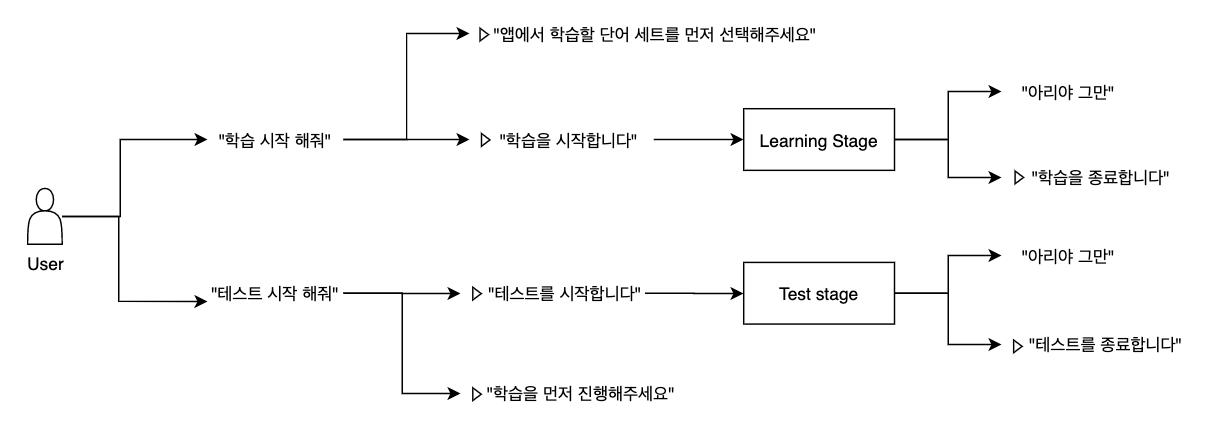
\includegraphics[width=\textwidth,height=6cm]{images/diagram_speaker.png}
%    \hfill
%    \caption{NUGU Speaker Diagram}
%\end{figure*}
\begin{enumerate}
    \item Learning Stage
    \begin{enumerate}
        \item When user says “학습 시작 해 줘”, the speaker answers “학습을 시작합니다.”
        \item If the user have not selected the word set to learn, the speaker answers “앱에서 학습할 단어 세트를 먼저 선택해 주세요.”
        \item The speaker fetches and gets the “current learning list” from the server and starts reading the words inside the list.
        \item The speaker reads words and the meaning 3 times in an interval of 2 seconds.
        \item After finishing reading the “current learning list”, it repeats the process as many time as the user set in the settings page of mobile application. 
        \item When the learning stage finishes, the speaker says “학습을 종료합니다”
        \item When the user says “아리야, 그만”, the speaker ends the process without saving the progress.
        \item When learning stage is interrupted by an unprecedented error, terminates the app.
        \item If the learning stage has been completed without any trouble, the speaker sends the sever “end signal”
        \item Users are enabled to start the learning stage as many time he/she wants.
    \end{enumerate}
    \item Test Stage
    \begin{enumerate}
        \item When user says “테스트 시작 해줘”, the speaker answers “테스트를 시작합니다.
        \item If the user says “테스트 시작 해줘” without finishing the learning stage, the speaker answers “학습을 먼저 진행해주세요”
        \item The speaker fetches the “to be tested word list” from the server and tests the user.
        \item The speaker reads the vocabulary and waits 10 seconds for the user input.
        \item The speaker sends the user input after processing it with NLP and determines if it is a correct answer or not.
        \item If the answer is wrong, red light flicks up, and green if not.
        \item If the user does not answer in the 10 waiting seconds, mark it as incorrect.
        \item After finishing the test stage, the speaker says “테스트를 종료합니다.”
        \item When the user says “아리야 그만” during the test stage, the speaker ends the process without saving the process.
        \item When the test stage is interrupted by an unprecedented error, terminates the app.
        \item If the test stage has been completed without any trouble, the speaker sends the server “end signal".
        \item The users are only able to test once for the specific word set. After the test stage, the “to-be-tested list” gets updated, and the user should move on to the next word set for learning.
    \end{enumerate}
\end{enumerate}


\subsection{Server}

\begin{enumerate}
    \item Mobile Application
    \begin{enumerate}
        \item In the server’s database, there are two lists which are “current-learning list” and “to-be-tested list”
        \item “To-be-tested list” comprises two parts; “new word list” and “review word list”. There are three columns in these lists, which are vocabulary, meaning, and forgetting rate.
        \item In the server’s database, word sets to be pre-included are saved.
        \item When user selects the word set to learn, server updates “current-learning list” and “to-be-tested list”
        \begin{enumerate}
            \item When the user chooses the word set that he/she never chose before, the chosen word set’s first sub-word set is copied into the “current-learning list”.
            \item In the first test stage, the “review word list” of the “to-be-tested list” remains blank.
            \item If the user chose the word set that he/she already learned before
            \begin{enumerate}
                \item If the latest progress is the learning stage, not the test stage, for example, if the user only learned, not tested chapter 4 of the TOEIC word set, copy the words in chapter 4 into “current-learning list” and “new word list” of “to-be-tested list”. “review word list” of the “to-be-tested list” gets comprised with words that have been selected via the human forgetting curve algorithm from the previous chapters.
                \item If the user finished testing, for example, if the user finished the testing stage of chapter 4 of TOEIC word set, and if he/she wishes to learn the previously learned word set again, copy chapter 5 words into “current-word list” and leave blank “new word list” of “to-be-tested list”. “Review word list” of “to-be-tested list” gets comprised of words that have been selected via the human forgetting curve algorithm from the previous chapters.
            \end{enumerate}
        \end{enumerate}
        \item If the user changes the word set before finishing the current word set, leave the current database, and make a new instance of “current-learning list” and “to-be-tested list”
        \item If the user adds a word set, sub-word set or word, add it into the server’s database.
        \begin{enumerate}
            \item If the user adds a word into a sub-word set that has not been learned before, just add vocabulary and meaning into the database, leaving the forgetting rate blank.
            \item If the user adds a new word into the sub-word set which has been learned, just add the vocabulary and meaning into the database, leaving the forgetting rate blank and copy the list into the “current-learning list”, and “new word list” of “to-be-tested lists”
            \item If the user adds a new word into a sub-word set that has been tested, apply the lowest forgetting rate, and adds it into the list with vocabulary and its meaning. This is reflected when the “to-be-tested list” gets updated.
        \end{enumerate}
        \item When the user deletes a word set, sub-word set or word, the words get deleted in the servers database.
    \end{enumerate}
    
    \item NUGU AI speaker
    \begin{enumerate}
        \item Learning Stage
        \begin{enumerate}
            \item When the user starts the learning stage, the server sends the speaker the “current-learning list”
            \item If the speaker gets interrupted by an unprecedented error, do not update the progress and sends the same “current-learning list” when the new learning stage begins.
            \item When the speaker sends the “end signal” of the learning stage, the checkbox in the mobile application changes into yellow, and copy the “current-learning list” into the “new word list” of “to-be-tested list”
            \item If the user learned any of the sub-word set, change the word set’s checkbox into yellow.
            \item If the “current-learning list” is empty, send an error message to the speaker. The speaker than says “학습할 단어 세트를 먼저 선택해 주세요.”
        \end{enumerate}
        \item Test Stage
        \begin{enumerate}
            \item When the user starts the test stage, the server sends the speaker “to-be-tested list”
            \item Speaker gets input from the user and determines if it is a correct answer or not. If it is a correct word, the forgetting rate rises, and remains the same if not. Every word in the “to-be-tested list” follows this procedure.
            \item The first tested word gets rated as the lowest rate of forgetting rate. As the learning goes on, words are tested repeatedly, and the forgetting rate gets raised if the user input is correct. The words with the highest forgetting rate are treated as saved in the long-term memory and not being tested again.
            \item If the speaker gets interrupted in the test stage via unprecedented error, do not save the progress and send the same “to-be-tested list” when the test stage begins.
            \item If the speaker sends the “end signal” of the test stage, changed the sub-word set’s checkbox into green. Moreover, the “new word list” in the “to-be-tested list gets flushed and updates the “review word list” of the “to-be-tested-list" regarding the forgetting rate, then update the “current-learning list” with the next words of the sub-word set. If the sub-word set is finished testing, the sub-word set’s checkbox changes into green.
            \item If the speaker sent the “end signal” of the test stage but there is not new sub-word set, change the checkbox of the word set into green. Empty the “current-learning list” and “to-be tested list”.
            \item If the “new word list” of the “to-be-tested list” is empty, the server sends the speaker an error message, and the speaker says “학습을 먼저 진행해 주세요.”
        \end{enumerate} 
    \end{enumerate}
\end{enumerate}






\section{Architecture Design \& Implementation}
    \subsection{Overall Architecture}
Brain Engraver consists of four modules. The first module is NUGU AI Speaker and Android Studio. This module is the front end of our application, which reacts with the user. The second module is the NUGU platform. It gets the voice input from the user and processes using its own ASR, NLU, NLG and TTS engine. Within the NUGU platform, there is "Play Builder" which enables us to add user utterance model and custom actions for it. Third module is HEROKU web sever, which is a PaaS(Platform as a Service). We deployed our application to HEROKU as a dynos, and uploaded the MySQL database along with it. For the database, since HEROKU does not support MySQL, we installed CelarDB MySQL Ignite to the HEROKU to process our original MySQL database. For the last module, we used AWS EC2(Linux Ubuntu Server 20.04). This module was used to test the software features and contructions of MySQL database. This AWS server was connected to the NUGU Platform directly for development purpose.
\begin{figure}[h]
    \centering
    \hfill
    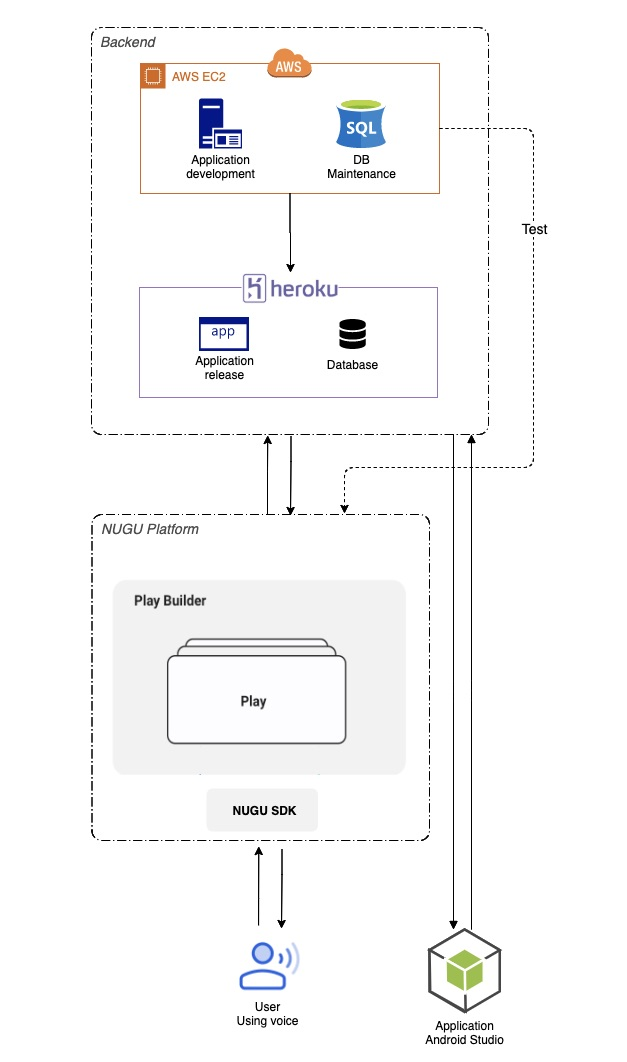
\includegraphics[width=8cm,height=15cm]{images/diagram1.jpeg}
    \hfill
    \caption{Overall Architecture}
\end{figure}

    \subsection{Directory organization}

    \begin{table}[htbp]
        \caption{Directory Organization}
        \begin{center}
        \begin{tabular}{ | c | c | c |} 
        \hline
        \textbf{\textit{Directory}}& \textbf{\textit{File name}}& \textbf{\textit{Module name}}\\
        \hline
        Brain-Engraver/app & \makecell{application.py \\ nugu.py \\ db.py \\ forgettingrate.py}& \makecell{AWS EC2 server \\ HEROKU server}\\
        \hline
        Brain-Engraver/db & \makecell{Brain\_Engraver.sql}& \makecell{AWS EC2 server \\ HEROKU server}  \\
        \hline\
        Brain-Engraver/server & \makecell{MANIFEST.in \\ Procfile \\ requirements.txt \\ setup.py}& \makecell{HEROKU server}  \\
        \hline\
        Brain-Engraver/doc & \makecell{main.tex}& \makecell{Documentation}\\
        \hline
        \makecell{Brain-Engraver/mobile\\App/java/com.example\\.brainengraver} & \makecell{AboutUs.java\\TOEICActivity.java\\TOEICChapter1Activity.java\\TOEICChapter2Activity.java\\TOEICChapter3Activity.java\\TOEFLActivity.java\\TOEFLChapter1Activity.java\\TOEFLChapter2Activity.java\\TOEFLChapter3Activity.java\\GREActivity.java\\GREChapter1Activity.java\\GREChapter2Activity.java\\GREChapter3Activity.java\\Login.java\\MainAcivity.java\\RegistrationActivity.java}& \makecell{Android Studio}\\
        \hline
        \makecell{Brain-Engraver/mobile\\App/res/drawable} & \makecell{ic\_aboutus.xml\\ic\_check.xml\\ic\_exam.xml\\ic\_home.xml\\ic\_launcher\_background.xml\\ic\_launcher\_foreground.xml\\ic\_logout.xml\\ic\_menu.xml\\ic\_more.xml\\ic\_previous.xml\\ic\_settings.xml\\round\_edittext.xml}& \makecell{Android Studio}\\
        \hline
        \makecell{Brain-Engraver/mobile\\App/res/font} & \makecell{poppins\_bold.xml\\poppins\_medium.xml}& \makecell{Android Studio}\\
        \hline
        \makecell{Brain-Engraver/mobile\\App/res/layout} & \makecell{activity\_about\_use.xml\\activity\_TOEIC.xml\\activity\_TOEIC\_chapter1.xml\\activity\_TOEIC\_chapter2.xml\\activity\_TOEIC\_chapter3.xml\\activity\_TOEFL.xml\\activity\_TOEFL\_chapter1.xml\\acitivity\_TOEFL\_chapter2.xml\\activity\_TOEFL\_chapter3.xml\\activity\_GRE.xml\\activity\_GRE\_chapter1.xml\\acitivity\_GRE\_chapter2.xml\\activity\_GRE\_chapter3.xml\\activity\_exam.xml\\activity\_login.xml\\activity\_main.xml\\main\_nav\_drawer.xml\\main\_toolbar.xml}& \makecell{Android Studio}\\
        \hline
        \makecell{Brain-Engraver/mobile\\App/res/values} & \makecell{arrays.xml\\colors.xml\\settings.xml\\}& \makecell{Android Studio}\\
        \hline
        \makecell{Brain-Engraver/mobile\\App/res/values\\themes} & \makecell{themes.xml\\themes\_dark.xml}& \makecell{Android Studio}\\
        \hline
        \end{tabular}
        \label{tab1}
        \end{center}
    \end{table}

    \begin{enumerate}
        \item MODULE 1: NUGU AI Speaker / Android Studio
        \begin{enumerate}
            \item Purpose
            \begin{itemize}
                \item When memorizing a vocabulary, it goes without saying that listening and reading the vocabulary is more effective than just looking. We decided to use NUGU AI Speaker because it enabled us to interact with the user using voice. Moreover, the fact that NUGU platform supports many pre-built actions and intent worked as one of the reason behind choosing the NUGU AI speaker.
                \item The user can use mobile application to sign in or sign up for their own "ForgettingRate" table.
                \item The user can check the spelling of the word on the mobile application.
            \end{itemize}
            \item Functionality
                \begin{itemize}
                    \item NUGU AI Speaker has microphone to get the user's voice and speaker to talk back to the user. It also has a volume up/down and mute/unmute button.
                \end{itemize}
        \end{enumerate}
        
        \item MODULE 2: NUGU Platform
            \begin{enumerate}
            \item Purpose
                \begin{itemize}
                    \item NUGU Platform is needed to connect NUGU AI Speaker with Brain Engraver on the server. We used the NUGU platform to assign keywords for intents and made specific HTTP POST requests to send to the server. After receiving the response from the server, it goes through specific action that we programmed such as testing the user.
                \end{itemize}
            \item Functionality
                \begin{itemize}
                    \item NUGU AI Speaker supports can process the user's voice with ASR(Automatic Speech Recognition), and it can understand the sentence's meaning with NLU(Natural Language Understanding). Moreover, it supports DM(Dialog Management) to send a request to our backend server. After getting the response from the server, by using NLG(Natural Language Generation) along with TTS(Text-to-Speech), it give the user output via natural language.
                \end{itemize}
            \end{enumerate}
            
        \item MODULE 3: HEROKU Web Server
            \begin{enumerate}
                \item Purpose
                    \begin{itemize}
                        \item We chose HEROKU web server to release our application because the releasing process is relatively simpler than other web server services. We originally chose AWS Elastic Beanstalk, but it did not support Python 3.8.3, and had several compatibility issues so we chose HEROKU instead. Moreover, since NUGU playbuilder has a server issue of connecting to the backend server, so using HEORKU, which can select to use HTTPS or HTTP, seemed like a wise choice.
                    \end{itemize}
                \item Functionality
                    \begin{itemize}
                        \item It is used to host the application to the web server. When using AWS EC2 Ubuntu server, the user had to configure every little steps in order to use Brain Engraver, but by using HEROKU, anyone can use the application without installing any libraries or plugins.
                    \end{itemize}
                \item Location of source code
                    \begin{itemize}
                        \item Brain-Engraver/app
                    \end{itemize}
                \item Class component: application.py
                    \begin{enumerate}
                        \item Choosing function
                            \begin{enumerate}
                                \item Choosing function is developed in the NUGU play builder with three branch actions. It goes through each action when one is finished. It is comprised of "chooseChapter", "chooseWordSet" and "chooseSubWordSet". Each action name is put behind the server's url.
                                \item chooseChapter()
                                    \begin{itemize}
                                        \item It receives action from the server with https://brainengraver.herokuapp.com:5\\500/chooseChapter post method. It replies the NUGU playbuilder blank response. This function is needed because the NUGU AI speaker has to ask the user "Which Chapter to learn? ("어떤 단어셋을 선택하시겠습니까?")" so that the user knows what to reply.
                                    \end{itemize}
                                \item chooseWordSet()
                                    \begin{itemize}
                                        \item It receives action from the server with https://brainengraver.herokuapp.com:5\\500/chooseWordSet post method. It stores the choosen wordset to the server, more specifically, in the nugu.py. After storing the value, it returns the choosen wordset's name such as "TOEIC", "TOEFL" to the NUGU playbuilder.
                                    \end{itemize}
                                \item chooseSubWordSet()
                                    \begin{itemize}
                                        \item It receives action from the server with https://brainengraver.herokuapp.com:5\\500/chooseSubWordSet post method. It stores the chosen subwordset from the user to the nugu.py located within the server. After storing the value, it returns the choosen subwordset's name such as "Chapter 1", "Chapter 2" and so on to the NUGU playbuilder.
                                    \end{itemize}
                                \item studyStart()
                                    \begin{itemize}
                                        \item It receives action from the server with https://brainengraver.herokuapp.com:5\\500/studyStart post method. It fetches the chosen wordset and subwordset from the nugu.py. This function firstly deletes the Study table from the MySQL database on the server, and updates the Study table with the words to learn today. Secondly, it marks the chosen chapter that it has been studied and initializes the forgetting rate to 0, and forgetting stage to 1.
                                    \end{itemize}
                                \item word\_1 to 15
                                    \begin{itemize}
                                        \item It receives action from the server with https://brainengraver.herokuapp.com:5\\500/word\_1~15 post method. This function returns specific word and its meaning. For example, word\_1() returns the first word from the chosen chapter.
                                    \end{itemize}
                                \item examStart()
                                    \begin{itemize}
                                        \item It receives action from the server with https://brainengraver.herokuapp.com:5\\500/examStart post method. It fetches the chosen wordset and subwordset. After fetching it, it firstly flushes the Exam table and gets the words that the user has been studied. Secondly, it updates the forgettingrate by calling the update\_forgettingRate() from the forgettingrate.py. Lastly, it updates the Exam table with the words that have low forgettingrate.
                                    \end{itemize}
                                \item question\_1 to 15()
                                    \begin{itemize}
                                        \item It receives action from the server with https://brainengraver.herokuapp.com:5\\500/answer\_1 to
                                        15. It revokes the question() function from the nugu.py and gives the user back the word to be tested by the NUGU AI Speaker. User then has to answer it's meaning to the NUGU AI Speaker.
                                    \end{itemize}
                                \item answer\_1 to 15()
                                    \begin{itemize}
                                        \item It receives action from the server with https://brainengraver.herokuapp.com:5\\500/answer\_1 to 15. It revokes the answer() function from the nugu.py and tells whether the user's answer is correct or not. After this, the function responds with "correctness(if the answer is correct, it is set to correct, and incorrect otherwise)" to the NUGU playbuilder.
                                        \end{itemize}
                            \end{enumerate}
                \item Class component: nugu.py
                    \begin{enumerate}
                        \item setWordSet()
                            \begin{itemize}
                                \item It stores the choosen wordset and subwordset to the global variable "wordset".
                            \end{itemize}
                        \item setSubWordSet()
                            \begin{itemize}
                                \item It stores the choosen subwordset to the global variable "subwordset".
                            \end{itemize}
                        \item study()
                            \begin{itemize}
                                \item It fetches the words to study from the study table in the database and returns the specific word and its meaning to the NUGU Playbuilder.
                            \end{itemize}
                        % \item finishstudy()
                        %     \begin{itemize}
                        %         \item 
                        %     \end{itemize}
                        \item question()
                            \begin{itemize}
                                \item It fetches the word to be tested from the db.py and responds to the server with the word.
                            \end{itemize}
                        \item answer()
                            \begin{itemize}
                                \item It receives the user's answer from the application.py and checks with the original meaning which is fetched from the database. If the user's answer is correct, it returns the server "correct" and "incorrect" otherwise. Furthermore, it calls the update\_forgettingStage() and update\_testTime() in the forgettingrate.py to update forgettingstage and forgettingrate for each answer.
                            \end{itemize}
                    \end{enumerate}
\begin{figure*}[h]
    \centering
    \hfill
    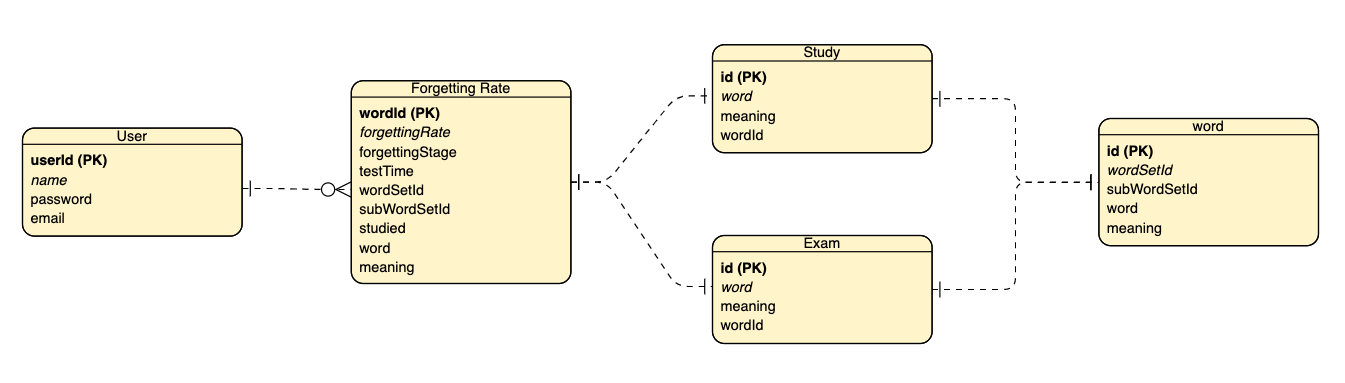
\includegraphics[width=\textwidth, height=7cm]{images/diagram2.png}
    \hfill
    \caption{Database}
\end{figure*}
                \item Class component: db.py
                    \begin{enumerate}
                        \item initDB()
                            \begin{itemize}
                                \item It returns pymysql.connect(hostname, port number, username, password, schema name, and charset).
                            \end{itemize}
                        \item getDB(query, parameter)
                            \begin{itemize}
                                \item It initializes database by calling initDB() and gets query, parameter from other functions and fetches return the rows from the specific table within database.
                            \end{itemize}
                        \item setDB()
                            \begin{itemize}
                                \item It initializes database by calling initDB() and gets query, parameter from other functions and sets the specific table within database.
                            \end{itemize}
                        \item getStudy()
                            \begin{itemize}
                                \item Sets the sql statement to select every data from Study table within database and callse getDB()
                            \end{itemize}
                        \item getAnswer(question\_id)
                            \begin{itemize}
                                \item Sets the sql statement to select specific word and meaning from Word table within database.
                            \end{itemize}
                        \item getExamWords(wordSetId, subWordSetId)
                            \begin{itemize}
                                \item Sets the sql statement to select 10 from the original test, and adds additional 5 words that is likely to be forgotten and returns the list of exam words.
                            \end{itemize}
                        \item setExamWords(word, meaning, wordId)
                            \begin{itemize}
                                \item Sets the sql statement to insert word, meaning and value to the table Exam in database and calls setDB().
                            \end{itemize}
                        \item deleteExam()
                            \begin{itemize}
                                \item Sets the sql statement to flush the Exam table in database and calls setDB().
                            \end{itemize}
                        \item getExam()
                            \begin{itemize}
                                \item Sets the sql statement to select every data from the Exam table in database and calls getDB().
                            \end{itemize}
                        \item getStudiedWords()
                            \begin{itemize}
                                \item Sets the sql statement to select only the data that has been studided from Word table in database and calls getDB().
                            \end{itemize}
                        \item getForgettingRateWords()
                            \begin{itemize}
                                \item Sets the sql statement to select word, meaning from the ForgettingRate table and calls the getDB().
                            \end{itemize}
                        \item insert\_ForgettingRate(word, meaning, wordId, wordSetId, subWordSetId)
                            \begin{itemize}
                                \item Sets the sql statement to insert studied words into the forgettingrate table in the database with default value, forgettingrate to 0 and forgettingstage to 0 , and calls the setDB().
                            \end{itemize}
                        \item deleteStudy()
                            \begin{itemize}
                                \item Sets the sql statement to flush the Study table in database and calls setDB().
                            \end{itemize}
                        \item getStudyWords(wordSetId, subWordSetId)
                            \begin{itemize}
                                \item Sets the sql statement to select the choosen wordset and subwordset's word and calls getDB().
                            \end{itemize}
                        \item setStudyWords(word, meaning, wordID)
                            \begin{itemize}
                                \item Sets the sql statement to insert studied words into the study table in database and calls setDB(). 
                            \end{itemize}
                    \end{enumerate}
                    %%%%%%%%%%%%%%%%%%%%%뽀게팅레이트.py 설명이요!!!!!
\begin{figure}[h]
    \centering
    \hfill
    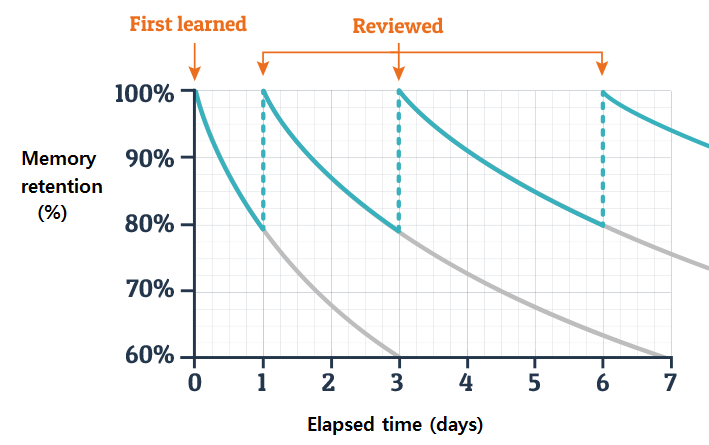
\includegraphics[width=9cm, height=6cm]{forgetting_curve.png}
    \hfill
    \caption{Ebbinghaus' forgetting curve}
\end{figure}
                \item Class component: forgettingrate.py
                    \begin{enumerate}
                        \item update\_testTime(answer)
                            \begin{itemize}
                                \item It sets the sql statement to update the testTime in forgettingrate table with time when the function is called and calls setDB().         
                            \end{itemize}
                        \item fx(testTime, forgettingStage)
                            \begin{itemize}
                                \item It calculates the forgettingrate according to the testtime and forgettingstage. The equation is from the Forgetting Curve of Ebbinghaus and the independent variable is the difference between testtime and time now. Lastly, it returns calculated forgettingrate.
                            \end{itemize}
                        \item cal\_forgettingRate(forgettingStage, testTime)
                            \begin{itemize}
                                \item It calculates the forgettingrate according to the forgettingstage and the return value of function fx. If the forgettingstage is 5, which means long-term memory, it returns the highest forgettingrate. If the forgettingrate is 1-4, which means short-term memory, it returns the forgettingrate calculated by function fx.   
                            \end{itemize}
                        \item update\_forgettingRate(answer)
                            \begin{itemize}
                                \item It sets the sql statement to update the forgettingrate from forgettingrate table with newly calculated forgettingrate. If a word has only been studied and has not been tested, it updates the forgetting rate with 0. Lastly, it calls setDB(). 
                            \end{itemize}
                        \item update\_forgettingStage(answer, correct)
                            \begin{itemize}
                                \item It sets the sql statement to update the forgettingstage according to "correct". If the user's answer is correct, the forgettingstage goes up. If the user's answer is wrong, the forgettingstage does not change.  
                            \end{itemize}
                        \item update\_SubWordSet\_studied(wordSetId, subWordSetId)
                            \begin{itemize}
                                \item It sets the sql statement to update studied field in word table with 1 and calls setDB().
                            \end{itemize}
                    \end{enumerate}
                
                \end{enumerate}
            \end{enumerate}
        \item MODULE 4: AWS EC2(Linux Ubuntu Server 20.04)
            \begin{enumerate}
                \item Purpose
                    \begin{itemize}
                        \item We used AWS EC2 Ubuntu server for our development process. We developed the beta program on the Ubuntu and connected it with NUGU Playbuilder for testing purpose. By using AWS EC2, we could add a function or fix the code without impacting the working version of the code.
                    \end{itemize}
                \item Founctionality
                    \begin{itemize}
                        \item Since it basically like renting a whole Ubuntu computer from Amazon, any type of experiments we wanted to do on Brain Engraver was possible. On top of this, we could configure our working environment just the way we planned before the coding process.
                    \end{itemize}
                \item Class component: same as HEROKY web server
            \end{enumerate}
        
        
    \end{enumerate}
    
    
\begin{figure*}[h]
    \centering
    \hfill
    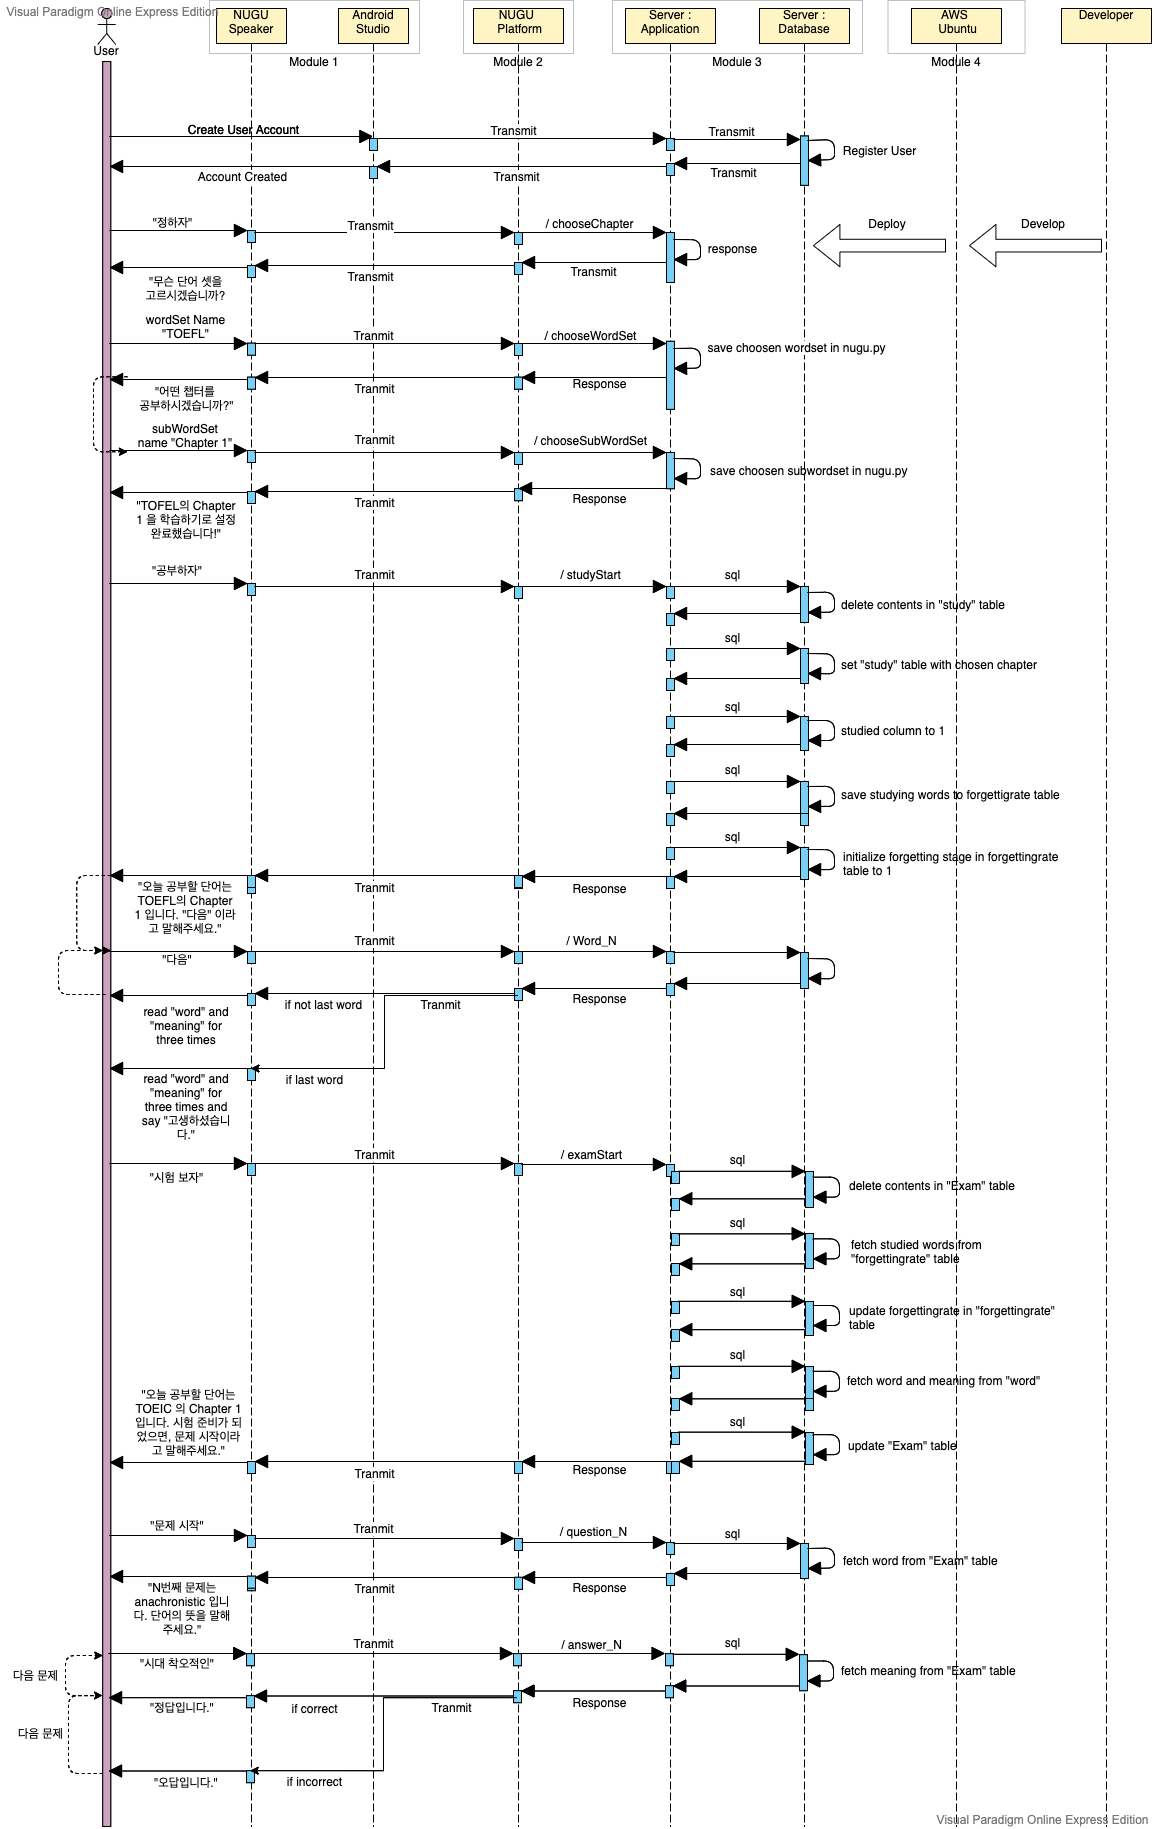
\includegraphics[width=\textwidth, height=24cm]{diagram2.png}
    \hfill
    \caption{Diagram}
    %\vspace{-40pt}
\end{figure*}
\section{Use Cases}
\begin{figure*}[h]
    \centering
    \hfill
    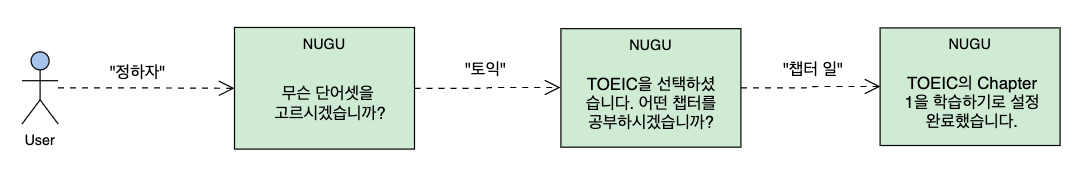
\includegraphics[width=\textwidth, height=3cm]{images/usecase1.png}
    \hfill
    \caption{Use case 1}
\end{figure*}
\begin{figure*}[h]
    \centering
    \hfill
    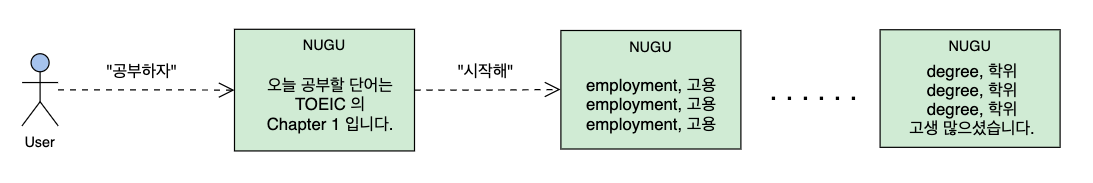
\includegraphics[width=\textwidth, height=3.5cm]{images/usecase2.png}
    \hfill
    \caption{Use case 2}
\end{figure*}
\begin{figure*}[h]
    \centering
    \hfill
    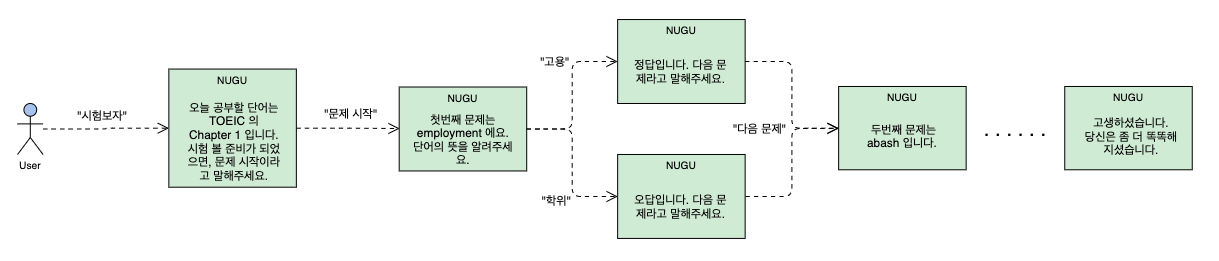
\includegraphics[width=\textwidth, height=4cm]{images/usecase3.png}
    \hfill
    \caption{Use case 3}
\end{figure*}
\begin{figure*}[h]
    \centering
    \hfill
    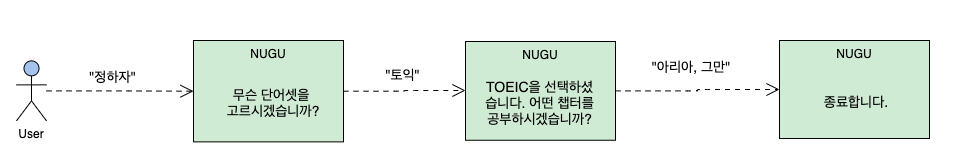
\includegraphics[width=\textwidth, height=3.5cm]{images/usecase4.png}
    \hfill
    \caption{Use case 4}
\end{figure*}
    \subsection{Installation}
        \begin{enumerate}
            \item The mobile application can be found in 'Google Play Store'. our application will be recommended when the user searches for certain keywords, such as 'English', 'learning', 'vocabulary', 'memorize'. Simple click button will install it to the user's mobile phone. 
            \item For the speaker, Brain Engraver is already installed in NUGU application(both Android and iOS). It can be found in the "Education / Kids" catetory under "NUGU PLAY".
            %여기에 사진 넣으면 좋지 않을까요...?!
        \end{enumerate}
    \subsection{Starting the application}
        \begin{enumerate}
            \item The user should first use the mobile application to sign up or sign in to get the token.
            \item The token is sent to the server, creating the token's own ForgettingRate table.
            \item When user launches the Brain Engraver application on the mobile phone, the login page will be shown. If the user does not have an account, user can create a new account using the sign-up button.
            \item In the NUGU Play"뇌새김" within the NUGU application, there is a sample voice interaction sentences for the user to try.
            \item When the user speaks "아리야, 뇌새김 시작해줘", the NUGU AI speaker says it is launched, and waits for the user to choose a certain function.
            %여기도 사진!!!
        \end{enumerate}
    \subsection{Choosing wordset}
        \begin{enumerate}
            \item When the user speaks "정하자", the NUGU AI Speaker starts the application and asks the user which chapter to choose. The user can choose the wordset "TOEIC" by speaking "토익", "토플" for "TOEFL", and "지얼이" for "GRE".
            \item if the user does not choose the correct chapter, the application terminates
        \end{enumerate}
    \subsection{Choosing Chapter}
        \begin{enumerate}
            \item After choosing the wordset to learn, NUGU AI Speaker automatically asks you to choose a chapter(Subwordset). The user can choose the chapter he/she wants by speaking "챕터 일", "챕터 이" and so on.
            \item if the user does not choose the correct chapter, the application terminates.
            \item when the word set and sub word set has been choosen by the user, the NUGU AI Speaker speaks "TOEIC(TOEFL or GRE) 의 Chapter 1(2 or 3)을 학습하기로 설정 완료했습니다!"
        \end{enumerate}
    \subsection{Learning stage}
        \begin{enumerate}
            \item After choosing the wordset and the chapter(Subwordset), the user starts the "study" function by simply speaking "공부하자".
            \item In the "study" function, which is the learning stage mentioned above in the specifications, NUGU AI speaker reads the word 3 times.
            \item In order to learn the next word, the user should say "다음".
            \item The "study" function terminates when the chosen chapter is finished.
            \item If the user wishes to interrupt during the process, the user can just say "아리아, 그만"
            \item The forgettingstage for each word in the selected chapter is initialized to 1.
        \end{enumerate}
        %%%%%%%%%%
        % 동희씨!!! 여기에 뽀게팅레이트 스테이지 이니셜라이징 되는거 적어주시면 될 것 같습니다!!!!
        %%%%%%%%%%
        
    \subsection{Test stage}
        \begin{enumerate}
        \item After finishing the learning stage, the user can start the test stage, "exam" function by "시험보자"
        \item Before starting "exam" function, forgettingrate is updated according to the time when the "exam" function is called.
        \item In the "exam" function, the user goes through total 15 words, which comprises 10 words that the user have just learned in the learning stage, and 5 words that is likely to be forgotten.
        \item 5 words are chosen by the Ebbinghaus's Forgetting Curve theory.
        \item The forgettingstage for each word is updated depending on the user's answer.
        \item The testtime for each word is updated with the time when the speaker received the user's answer.
        \end{enumerate}
    
    \subsection{Check word on mobile application}
    \begin{enumerate}
        \item The user can always check the word and its' meaning from the mobile application.
        \item To check the wordset, click the menu above, click  Word Set, click word set such as TOEIC and click sub word set such as Chapter1.
    \end{enumerate}
    % %%%%%%%%%
    % 동희씨!!! 여기에는 뽀게팅 레이트 업데이트하는 부분 적어주시면 될 것 같아요!!!!!
    % %%%%%%%%%
    \subsection{Interrupt/terminate function}
        \begin{enumerate}
        \item In order to finish the application during the process of "learning stage" or "test stage", user should say "아리아, 뇌새김 그만" or "아리아, 뇌새김 닫아줘"
        \item When user says "아리아 , 그만", the application terminates without saving its progress.
        \item When NUGU speaker is in the session waiting for the user to speak, user can just say "그만" to terminate the process.
        \end{enumerate}
    \subsection{Error}
        The problem behind NUGU playbuilder is that it can only map the specific word to the intent. This means that even though the intent's name is different(same with entity's name and action's name), the invocation word or the word that NUGU spekaer learned cannot be the same. On top of this, Intent created by us was prohibited to use in multiple actions unless its a one -continuously-starting branch action. Originally, we wanted to make a "Exam Function" that only tested the user with the words that the user just learnt, and a "Forgetting Rate Exam Function" to test only the words that the user is likely to forgotten. So naturally, since NUGU playbuilder's restrictions forced us to merge the two "Exam Function" and "Forgetting Rate Function" together. To illustrate a light on the matter, we created two actions for "Exam Function" and "Forgetting Rate Exam Function". Since only one entity type can be mapped to one action, so we had to create two different named entity types named "Answer" and "Forgetting Rate Answer". These two entity types were mapped to each intents, and those intents consists of the meaning of the words. When we ran the program and tested, NUGU playbuilder did not know what request to send, so it did not work. By this reason, we had no choice to merge these two "Exam Function" and "Forgetting Rate Function" together.
        There were also a problem even when we merged these two actions. The problem was that when user started the exam action for the first time, there would be only 10 questions that the user have learned and 5 blank words that was supposed to be "likely-to-be-forgotten words". Consequently, error occured in the first test. So, in order to solve this problem, we had no choice but to increment 5 more words to the TOEIC's chapter 1. By doing this, on the first exam, NUGU playbuilder gave the test with 15 words that had been learned by the user, and on the second exam, NUGU playbuilder gave 10 just-learned words and 5 likely-to-be-forgotten words.
        \begin{enumerate}
            \item When the user's first test is not TOEIC's chapter 1
            \begin{enumerate}
                \item Error will not occur in the "learning stage"
                \item Error will occur in the 11th question of the "test stage"
                \item When the error occurs, the application will terminate itself
                \item order to avoid this error, study chapter 1 and take the chapter 1's exam. Afterwords, the error does not occur again.
            \end{enumerate}
            \item When the user says things that Brain Engraver cannot understand
            \begin{enumerate}
                \item When user speaks repeatedly the things Brain Engraver cannot understand, the application gets terminated.
            \end{enumerate}
            \item When the user does not speak
            \begin{enumerate}
                \item When the user does not speak during the listening session of the NUGU AI speaker, the application gets terminated.
            \end{enumerate}
            \item NUGU Platform server error
            \begin{enumerate}
                \item From time to time, NUGU server misacts and sends strange server requests. There are serveral types of nugu server errors that we found. The first one is that even if we change the backend server to another one and save the changes, the NUGU platform sometimes send the request to the previous backend server. Moreover, since our program is based on numerous branch actions, NUGU platform sometimes gets confused and sends previous action's request to the current action. When this kind of error happens, we figured out that waiting is the answer. We believe that it has something to do with ACKs comming late.
            \end{enumerate}
    \end{enumerate}




    % \begin{enumerate}
    % \item 
    % \item 
    % \item 
    % \item 
    % \item 
    % \end{enumerate}









% The IEEEtran class file is used to format your paper and style the text. All margins, 
% column widths, line spaces, and text fonts are prescribed; please do not 
% alter them. You may note peculiarities. For example, the head margin
% measures proportionately more than is customary. This measurement 
% and others are deliberate, using specifications that anticipate your paper 
% as one part of the entire proceedings, and not as an independent document. 
% Please do not revise any of the current designations.

% \section{Prepare Your Paper Before Styling}
% Before you begin to format your paper, first write and save the content as a 
% separate text file. Complete all content and organizational editing before 
% formatting. Please note sections \ref{AA}--\ref{SCM} below for more information on 
% proofreading, spelling and grammar.

% Keep your text and graphic files separate until after the text has been 
% formatted and styled. Do not number text heads---{\LaTeX} will do that 
% for you.

% \subsection{Abbreviations and Acronyms}\label{AA}
% Define abbreviations and acronyms the first time they are used in the text, 
% even after they have been defined in the abstract. Abbreviations such as 
% IEEE, SI, MKS, CGS, ac, dc, and rms do not have to be defined. Do not use 
% abbreviations in the title or heads unless they are unavoidable.

% \subsection{Units}
% \begin{itemize}
% \item Use either SI (MKS) or CGS as primary units. (SI units are encouraged.) English units may be used as secondary units (in parentheses). An exception would be the use of English units as identifiers in trade, such as ``3.5-inch disk drive''.
% \item Avoid combining SI and CGS units, such as current in amperes and magnetic field in oersteds. This often leads to confusion because equations do not balance dimensionally. If you must use mixed units, clearly state the units for each quantity that you use in an equation.
% \item Do not mix complete spellings and abbreviations of units: ``Wb/m\textsuperscript{2}'' or ``webers per square meter'', not ``webers/m\textsuperscript{2}''. Spell out units when they appear in text: ``. . . a few henries'', not ``. . . a few H''.
% \item Use a zero before decimal points: ``0.25'', not ``.25''. Use ``cm\textsuperscript{3}'', not ``cc''.)
% \end{itemize}

% \subsection{Equations}
% Number equations consecutively. To make your 
% equations more compact, you may use the solidus (~/~), the exp function, or 
% appropriate exponents. Italicize Roman symbols for quantities and variables, 
% but not Greek symbols. Use a long dash rather than a hyphen for a minus 
% sign. Punctuate equations with commas or periods when they are part of a 
% sentence, as in:
% \begin{equation}
% a+b=\gamma\label{eq}
% \end{equation}

% Be sure that the 
% symbols in your equation have been defined before or immediately following 
% the equation. Use ``\eqref{eq}'', not ``Eq.~\eqref{eq}'' or ``equation \eqref{eq}'', except at 
% the beginning of a sentence: ``Equation \eqref{eq} is . . .''

% \subsection{\LaTeX-Specific Advice}

% Please use ``soft'' (e.g., \verb|\eqref{Eq}|) cross references instead
% of ``hard'' references (e.g., \verb|(1)|). That will make it possible
% to combine sections, add equations, or change the order of figures or
% citations without having to go through the file line by line.

% Please don't use the \verb|{eqnarray}| equation environment. Use
% \verb|{align}| or \verb|{IEEEeqnarray}| instead. The \verb|{eqnarray}|
% environment leaves unsightly spaces around relation symbols.

% Please note that the \verb|{subequations}| environment in {\LaTeX}
% will increment the main equation counter even when there are no
% equation numbers displayed. If you forget that, you might write an
% article in which the equation numbers skip from (17) to (20), causing
% the copy editors to wonder if you've discovered a new method of
% counting.

% {\BibTeX} does not work by magic. It doesn't get the bibliographic
% data from thin air but from .bib files. If you use {\BibTeX} to produce a
% bibliography you must send the .bib files. 

% {\LaTeX} can't read your mind. If you assign the same label to a
% subsubsection and a table, you might find that Table I has been cross
% referenced as Table IV-B3. 

% {\LaTeX} does not have precognitive abilities. If you put a
% \verb|\label| command before the command that updates the counter it's
% supposed to be using, the label will pick up the last counter to be
% cross referenced instead. In particular, a \verb|\label| command
% should not go before the caption of a figure or a table.

% Do not use \verb|\nonumber| inside the \verb|{array}| environment. It
% will not stop equation numbers inside \verb|{array}| (there won't be
% any anyway) and it might stop a wanted equation number in the
% surrounding equation.

% \subsection{Some Common Mistakes}\label{SCM}
% \begin{itemize}
% \item The word ``data'' is plural, not singular.
% \item The subscript for the permeability of vacuum $\mu_{0}$, and other common scientific constants, is zero with subscript formatting, not a lowercase letter ``o''.
% \item In American English, commas, semicolons, periods, question and exclamation marks are located within quotation marks only when a complete thought or name is cited, such as a title or full quotation. When quotation marks are used, instead of a bold or italic typeface, to highlight a word or phrase, punctuation should appear outside of the quotation marks. A parenthetical phrase or statement at the end of a sentence is punctuated outside of the closing parenthesis (like this). (A parenthetical sentence is punctuated within the parentheses.)
% \item A graph within a graph is an ``inset'', not an ``insert''. The word alternatively is preferred to the word ``alternately'' (unless you really mean something that alternates).
% \item Do not use the word ``essentially'' to mean ``approximately'' or ``effectively''.
% \item In your paper title, if the words ``that uses'' can accurately replace the word ``using'', capitalize the ``u''; if not, keep using lower-cased.
% \item Be aware of the different meanings of the homophones ``affect'' and ``effect'', ``complement'' and ``compliment'', ``discreet'' and ``discrete'', ``principal'' and ``principle''.
% \item Do not confuse ``imply'' and ``infer''.
% \item The prefix ``non'' is not a word; it should be joined to the word it modifies, usually without a hyphen.
% \item There is no period after the ``et'' in the Latin abbreviation ``et al.''.
% \item The abbreviation ``i.e.'' means ``that is'', and the abbreviation ``e.g.'' means ``for example''.
% \end{itemize}
% An excellent style manual for science writers is \cite{b7}.

% \subsection{Authors and Affiliations}
% \textbf{The class file is designed for, but not limited to, six authors.} A 
% minimum of one author is required for all conference articles. Author names 
% should be listed starting from left to right and then moving down to the 
% next line. This is the author sequence that will be used in future citations 
% and by indexing services. Names should not be listed in columns nor group by 
% affiliation. Please keep your affiliations as succinct as possible (for 
% example, do not differentiate among departments of the same organization).

% \subsection{Identify the Headings}
% Headings, or heads, are organizational devices that guide the reader through 
% your paper. There are two types: component heads and text heads.

% Component heads identify the different components of your paper and are not 
% topically subordinate to each other. Examples include Acknowledgments and 
% References and, for these, the correct style to use is ``Heading 5''. Use 
% ``figure caption'' for your Figure captions, and ``table head'' for your 
% table title. Run-in heads, such as ``Abstract'', will require you to apply a 
% style (in this case, italic) in addition to the style provided by the drop 
% down menu to differentiate the head from the text.

% Text heads organize the topics on a relational, hierarchical basis. For 
% example, the paper title is the primary text head because all subsequent 
% material relates and elaborates on this one topic. If there are two or more 
% sub-topics, the next level head (uppercase Roman numerals) should be used 
% and, conversely, if there are not at least two sub-topics, then no subheads 
% should be introduced.

% \subsection{Figures and Tables}
% \paragraph{Positioning Figures and Tables} Place figures and tables at the top and 
% bottom of columns. Avoid placing them in the middle of columns. Large 
% figures and tables may span across both columns. Figure captions should be 
% below the figures; table heads should appear above the tables. Insert 
% figures and tables after they are cited in the text. Use the abbreviation 
% ``Fig.~\ref{fig}'', even at the beginning of a sentence.

% \begin{table}[htbp]
% \caption{Table Type Styles}
% \begin{center}
% \begin{tabular}{|c|c|c|c|}
% \hline
% \textbf{Table}&\multicolumn{3}{|c|}{\textbf{Table Column Head}} \\
% \cline{2-4} 
% \textbf{Head} & \textbf{\textit{Table column subhead}}& \textbf{\textit{Subhead}}& \textbf{\textit{Subhead}} \\
% \hline
% copy& More table copy$^{\mathrm{a}}$& &  \\
% \hline
% \multicolumn{4}{l}{$^{\mathrm{a}}$Sample of a Table footnote.}
% \end{tabular}
% \label{tab1}
% \end{center}
% \end{table}

% \begin{figure}[htbp]
% \centerline{\includegraphics{fig1.png}}
% \caption{Example of a figure caption.}
% \label{fig}
% \end{figure}

% Figure Labels: Use 8 point Times New Roman for Figure labels. Use words 
% rather than symbols or abbreviations when writing Figure axis labels to 
% avoid confusing the reader. As an example, write the quantity 
% ``Magnetization'', or ``Magnetization, M'', not just ``M''. If including 
% units in the label, present them within parentheses. Do not label axes only 
% with units. In the example, write ``Magnetization (A/m)'' or ``Magnetization 
% \{A[m(1)]\}'', not just ``A/m''. Do not label axes with a ratio of 
% quantities and units. For example, write ``Temperature (K)'', not 
% ``Temperature/K''.

% \section*{Acknowledgment}

% The preferred spelling of the word ``acknowledgment'' in America is without 
% an ``e'' after the ``g''. Avoid the stilted expression ``one of us (R. B. 
% G.) thanks $\ldots$''. Instead, try ``R. B. G. thanks$\ldots$''. Put sponsor 
% acknowledgments in the unnumbered footnote on the first page.

% \section*{References}

% Please number citations consecutively within brackets \cite{b1}. The 
% sentence punctuation follows the bracket \cite{b2}. Refer simply to the reference 
% number, as in \cite{b3}---do not use ``Ref. \cite{b3}'' or ``reference \cite{b3}'' except at 
% the beginning of a sentence: ``Reference \cite{b3} was the first $\ldots$''

% Number footnotes separately in superscripts. Place the actual footnote at 
% the bottom of the column in which it was cited. Do not put footnotes in the 
% abstract or reference list. Use letters for table footnotes.

% Unless there are six authors or more give all authors' names; do not use 
% ``et al.''. Papers that have not been published, even if they have been 
% submitted for publication, should be cited as ``unpublished'' \cite{b4}. Papers 
% that have been accepted for publication should be cited as ``in press'' \cite{b5}. 
% Capitalize only the first word in a paper title, except for proper nouns and 
% element symbols.

% For papers published in translation journals, please give the English 
% citation first, followed by the original foreign-language citation \cite{b6}.

% \begin{thebibliography}{00}
% \bibitem{b1} G. Eason, B. Noble, and I. N. Sneddon, ``On certain integrals of Lipschitz-Hankel type involving products of Bessel functions,'' Phil. Trans. Roy. Soc. London, vol. A247, pp. 529--551, April 1955.
% \bibitem{b2} J. Clerk Maxwell, A Treatise on Electricity and Magnetism, 3rd ed., vol. 2. Oxford: Clarendon, 1892, pp.68--73.
% \bibitem{b3} I. S. Jacobs and C. P. Bean, ``Fine particles, thin films and exchange anisotropy,'' in Magnetism, vol. III, G. T. Rado and H. Suhl, Eds. New York: Academic, 1963, pp. 271--350.
% \bibitem{b4} K. Elissa, ``Title of paper if known,'' unpublished.
% \bibitem{b5} R. Nicole, ``Title of paper with only first word capitalized,'' J. Name Stand. Abbrev., in press.
% \bibitem{b6} Y. Yorozu, M. Hirano, K. Oka, and Y. Tagawa, ``Electron spectroscopy studies on magneto-optical media and plastic substrate interface,'' IEEE Transl. J. Magn. Japan, vol. 2, pp. 740--741, August 1987 [Digests 9th Annual Conf. Magnetics Japan, p. 301, 1982].
% \bibitem{b7} M. Young, The Technical Writer's Handbook. Mill Valley, CA: University Science, 1989.
% \end{thebibliography}
% \vspace{12pt}
% \color{red}
% IEEE conference templates contain guidance text for composing and formatting conference papers. Please ensure that all template text is removed from your conference paper prior to submission to the conference. Failure to remove the template text from your paper may result in your paper not being published.

\end{document}
